\documentclass[twoside]{book}

% Packages required by doxygen
\usepackage{fixltx2e}
\usepackage{calc}
\usepackage{doxygen}
\usepackage[export]{adjustbox} % also loads graphicx
\usepackage{graphicx}
\usepackage[utf8]{inputenc}
\usepackage{makeidx}
\usepackage{multicol}
\usepackage{multirow}
\PassOptionsToPackage{warn}{textcomp}
\usepackage{textcomp}
\usepackage[nointegrals]{wasysym}
\usepackage[table]{xcolor}

% Font selection
\usepackage[T1]{fontenc}
\usepackage[scaled=.90]{helvet}
\usepackage{courier}
\usepackage{amssymb}
\usepackage{sectsty}
\renewcommand{\familydefault}{\sfdefault}
\allsectionsfont{%
  \fontseries{bc}\selectfont%
  \color{darkgray}%
}
\renewcommand{\DoxyLabelFont}{%
  \fontseries{bc}\selectfont%
  \color{darkgray}%
}
\newcommand{\+}{\discretionary{\mbox{\scriptsize$\hookleftarrow$}}{}{}}

% Page & text layout
\usepackage{geometry}
\geometry{%
  a4paper,%
  top=2.5cm,%
  bottom=2.5cm,%
  left=2.5cm,%
  right=2.5cm%
}
\tolerance=750
\hfuzz=15pt
\hbadness=750
\setlength{\emergencystretch}{15pt}
\setlength{\parindent}{0cm}
\setlength{\parskip}{0.2cm}
\makeatletter
\renewcommand{\paragraph}{%
  \@startsection{paragraph}{4}{0ex}{-1.0ex}{1.0ex}{%
    \normalfont\normalsize\bfseries\SS@parafont%
  }%
}
\renewcommand{\subparagraph}{%
  \@startsection{subparagraph}{5}{0ex}{-1.0ex}{1.0ex}{%
    \normalfont\normalsize\bfseries\SS@subparafont%
  }%
}
\makeatother

% Headers & footers
\usepackage{fancyhdr}
\pagestyle{fancyplain}
\fancyhead[LE]{\fancyplain{}{\bfseries\thepage}}
\fancyhead[CE]{\fancyplain{}{}}
\fancyhead[RE]{\fancyplain{}{\bfseries\leftmark}}
\fancyhead[LO]{\fancyplain{}{\bfseries\rightmark}}
\fancyhead[CO]{\fancyplain{}{}}
\fancyhead[RO]{\fancyplain{}{\bfseries\thepage}}
\fancyfoot[LE]{\fancyplain{}{}}
\fancyfoot[CE]{\fancyplain{}{}}
\fancyfoot[RE]{\fancyplain{}{\bfseries\scriptsize Generated on Wed Apr 15 2015 17\+:30\+:32 for Server D\+N\+C by Doxygen }}
\fancyfoot[LO]{\fancyplain{}{\bfseries\scriptsize Generated on Wed Apr 15 2015 17\+:30\+:32 for Server D\+N\+C by Doxygen }}
\fancyfoot[CO]{\fancyplain{}{}}
\fancyfoot[RO]{\fancyplain{}{}}
\renewcommand{\footrulewidth}{0.4pt}
\renewcommand{\chaptermark}[1]{%
  \markboth{#1}{}%
}
\renewcommand{\sectionmark}[1]{%
  \markright{\thesection\ #1}%
}

% Indices & bibliography
\usepackage{natbib}
\usepackage[titles]{tocloft}
\setcounter{tocdepth}{3}
\setcounter{secnumdepth}{5}
\makeindex

% Hyperlinks (required, but should be loaded last)
\usepackage{ifpdf}
\ifpdf
  \usepackage[pdftex,pagebackref=true]{hyperref}
\else
  \usepackage[ps2pdf,pagebackref=true]{hyperref}
\fi
\hypersetup{%
  colorlinks=true,%
  linkcolor=blue,%
  citecolor=blue,%
  unicode%
}

% Custom commands
\newcommand{\clearemptydoublepage}{%
  \newpage{\pagestyle{empty}\cleardoublepage}%
}


%===== C O N T E N T S =====

\begin{document}

% Titlepage & ToC
\hypersetup{pageanchor=false,
             bookmarks=true,
             bookmarksnumbered=true,
             pdfencoding=unicode
            }
\pagenumbering{roman}
\begin{titlepage}
\vspace*{7cm}
\begin{center}%
{\Large Server D\+N\+C \\[1ex]\large 1.\+0 }\\
\vspace*{1cm}
{\large Generated by Doxygen 1.8.9.1}\\
\vspace*{0.5cm}
{\small Wed Apr 15 2015 17:30:32}\\
\end{center}
\end{titlepage}
\clearemptydoublepage
\tableofcontents
\clearemptydoublepage
\pagenumbering{arabic}
\hypersetup{pageanchor=true}

%--- Begin generated contents ---
\chapter{D\+N\+C}
\label{md__home_sidya__pycharm_projects__d_n_c_serveur__r_e_a_d_m_e}
\hypertarget{md__home_sidya__pycharm_projects__d_n_c_serveur__r_e_a_d_m_e}{}
serveur

Requierement \+: -\/$>$ python 3.\+4 
\chapter{Namespace Index}
\section{Namespace List}
Here is a list of all namespaces with brief descriptions\+:\begin{DoxyCompactList}
\item\contentsline{section}{\hyperlink{namespace_log}{Log} \\*Module \hyperlink{namespace_log}{Log} }{\pageref{namespace_log}}{}
\item\contentsline{section}{\hyperlink{namespace_server}{Server} \\*Module server }{\pageref{namespace_server}}{}
\end{DoxyCompactList}

\chapter{Hierarchical Index}
\section{Class Hierarchy}
This inheritance list is sorted roughly, but not completely, alphabetically\+:\begin{DoxyCompactList}
\item \contentsline{section}{Log.\+bcolors}{\pageref{class_log_1_1bcolors}}{}
\item Filter\begin{DoxyCompactList}
\item \contentsline{section}{Log.\+Single\+Level\+Filter}{\pageref{class_log_1_1_single_level_filter}}{}
\end{DoxyCompactList}
\item \contentsline{section}{Log.\+lvl}{\pageref{class_log_1_1lvl}}{}
\item object\begin{DoxyCompactList}
\item \contentsline{section}{Log.\+Log}{\pageref{class_log_1_1_log}}{}
\end{DoxyCompactList}
\end{DoxyCompactList}

\chapter{Class Index}
\section{Class List}
Here are the classes, structs, unions and interfaces with brief descriptions\+:\begin{DoxyCompactList}
\item\contentsline{section}{\hyperlink{class_log_1_1bcolors}{Log.\+bcolors} \\*Define constant color value for different level }{\pageref{class_log_1_1bcolors}}{}
\item\contentsline{section}{\hyperlink{class_log_1_1_log}{Log.\+Log} \\*\hyperlink{class_log_1_1_log}{Log} Manager }{\pageref{class_log_1_1_log}}{}
\item\contentsline{section}{\hyperlink{class_log_1_1lvl}{Log.\+lvl} \\*Define constant value for level utils }{\pageref{class_log_1_1lvl}}{}
\item\contentsline{section}{\hyperlink{class_log_1_1_single_level_filter}{Log.\+Single\+Level\+Filter} \\*Filter for one level }{\pageref{class_log_1_1_single_level_filter}}{}
\end{DoxyCompactList}

\chapter{File Index}
\section{File List}
Here is a list of all files with brief descriptions\+:\begin{DoxyCompactList}
\item\contentsline{section}{/home/sidya/\+Pycharm\+Projects/\+D\+N\+C/serveur/\hyperlink{_log_8py}{Log.\+py} }{\pageref{_log_8py}}{}
\item\contentsline{section}{/home/sidya/\+Pycharm\+Projects/\+D\+N\+C/serveur/\hyperlink{_server_8py}{Server.\+py} }{\pageref{_server_8py}}{}
\end{DoxyCompactList}

\chapter{Namespace Documentation}
\hypertarget{namespace_log}{}\section{Log Namespace Reference}
\label{namespace_log}\index{Log@{Log}}


Module \hyperlink{namespace_log}{Log}.  


\subsection*{Classes}
\begin{DoxyCompactItemize}
\item 
class \hyperlink{class_log_1_1bcolors}{bcolors}
\begin{DoxyCompactList}\small\item\em Define constant color value for different level. \end{DoxyCompactList}\item 
class \hyperlink{class_log_1_1_log}{Log}
\begin{DoxyCompactList}\small\item\em \hyperlink{class_log_1_1_log}{Log} Manager. \end{DoxyCompactList}\item 
class \hyperlink{class_log_1_1lvl}{lvl}
\begin{DoxyCompactList}\small\item\em Define constant value for level utils. \end{DoxyCompactList}\item 
class \hyperlink{class_log_1_1_single_level_filter}{Single\+Level\+Filter}
\begin{DoxyCompactList}\small\item\em Filter for one level. \end{DoxyCompactList}\end{DoxyCompactItemize}


\subsection{Detailed Description}
Module \hyperlink{namespace_log}{Log}. 
\hypertarget{namespace_server}{}\section{Server Namespace Reference}
\label{namespace_server}\index{Server@{Server}}


Module server.  


\subsection*{Functions}
\begin{DoxyCompactItemize}
\item 
def \hyperlink{namespace_server_a3b6f7f7679d98f214467d05da4618a0c}{main} ()
\begin{DoxyCompactList}\small\item\em Load Configuration and Start the \hyperlink{namespace_server}{Server}. \end{DoxyCompactList}\item 
def \hyperlink{namespace_server_a5956f54107dc04f2c1700fcf62f1afc9}{handle\+\_\+connection} (connection, client\+\_\+address)
\begin{DoxyCompactList}\small\item\em Handle a connection from a client. \end{DoxyCompactList}\item 
def \hyperlink{namespace_server_a8965f4e84689d4e2b198091f0383fd41}{handle\+\_\+request} (connection, data)
\begin{DoxyCompactList}\small\item\em Handle a request. \end{DoxyCompactList}\item 
def \hyperlink{namespace_server_a5b7286b84051e8f089e78cec5276027f}{broadcast\+\_\+message} (connection, message)
\begin{DoxyCompactList}\small\item\em Broadcast a message to all the users connected except to the sender of the request. \end{DoxyCompactList}\item 
def \hyperlink{namespace_server_a79e61c36bfba574632384d7c95f687e8}{user\+\_\+list\+\_\+active} (connection)
\begin{DoxyCompactList}\small\item\em Send the list of enable user. \end{DoxyCompactList}\item 
def \hyperlink{namespace_server_a616374a08f1e1cd1c4fa745e10af349a}{user\+\_\+list\+\_\+away} (connection)
\begin{DoxyCompactList}\small\item\em Send the list of disable user. \end{DoxyCompactList}\item 
def \hyperlink{namespace_server_a59bc6f10d51dddca1906c85fdac1cc62}{change\+\_\+name} (connection, pseudo)
\begin{DoxyCompactList}\small\item\em Change the nickname of the user. \end{DoxyCompactList}\item 
def \hyperlink{namespace_server_aedccc2662d6bc5892f70e48009ed1b59}{new\+\_\+name} (connection, pseudo)
\begin{DoxyCompactList}\small\item\em Affect the nickname of the user for the first time. \end{DoxyCompactList}\item 
def \hyperlink{namespace_server_a46ba24f249f2961ada72160f9a9ba9b8}{ask\+\_\+private\+\_\+message} (connection, pseudo)
\begin{DoxyCompactList}\small\item\em Ask for a private discussion between the sender of the request and the pseudo. \end{DoxyCompactList}\item 
def \hyperlink{namespace_server_a1879fdb42898934db420d6c225db536e}{accept\+\_\+private\+\_\+message} (connection, pseudo)
\begin{DoxyCompactList}\small\item\em Accept a private discussion. \end{DoxyCompactList}\item 
def \hyperlink{namespace_server_a1ccbd55ee3033925a2b1ef2716dd0829}{reject\+\_\+private\+\_\+message} (connection, pseudo)
\begin{DoxyCompactList}\small\item\em Reject a private discussion. \end{DoxyCompactList}\item 
def \hyperlink{namespace_server_a5605c682f147e7cf9018ac02bb089989}{private\+\_\+message} (connection, pseudo, msg)
\begin{DoxyCompactList}\small\item\em Send a private message if a private discussion had been accepted. \end{DoxyCompactList}\item 
def \hyperlink{namespace_server_a2ddcf35a85844615fa31e72f6dcc52b0}{ask\+\_\+file} (connection, pseudo, file)
\begin{DoxyCompactList}\small\item\em Ask for a file transfer between the sender of the request and the pseudo. \end{DoxyCompactList}\item 
def \hyperlink{namespace_server_a0f21810c2b82ea1a98725185d2f3a70a}{accept\+\_\+file} (connection, pseudo, file, port)
\begin{DoxyCompactList}\small\item\em Accept a file transfer. \end{DoxyCompactList}\item 
def \hyperlink{namespace_server_a7b5be6de60d79f607c206c3675166301}{reject\+\_\+file} (connection, pseudo, file)
\begin{DoxyCompactList}\small\item\em Reject a file transfer. \end{DoxyCompactList}\item 
def \hyperlink{namespace_server_a114698f1955c3ff109f9fbbc1df306fa}{enable\+\_\+user} (connection)
\begin{DoxyCompactList}\small\item\em Enable user. \end{DoxyCompactList}\item 
def \hyperlink{namespace_server_af20de30ab901173d2bc8f58da7c05c25}{disable\+\_\+user} (connection)
\begin{DoxyCompactList}\small\item\em Disable user. \end{DoxyCompactList}\item 
def \hyperlink{namespace_server_af73d203b1f93b0f4014456fb52c7626a}{quit\+\_\+user} (connection)
\begin{DoxyCompactList}\small\item\em Disconnect user. \end{DoxyCompactList}\item 
def \hyperlink{namespace_server_a23b4ef94218cf46a4a1af4ed37c5278b}{get\+\_\+connection\+\_\+by\+\_\+pseudo} (pseudo)
\begin{DoxyCompactList}\small\item\em Get the socket descriptor by a pseudo. \end{DoxyCompactList}\end{DoxyCompactItemize}
\subsection*{Variables}
\begin{DoxyCompactItemize}
\item 
int \hyperlink{namespace_server_ad80a48b2e2123c1442355c35e9a12180}{U\+S\+E\+R\+L\+I\+S\+T\+\_\+\+E\+N\+A\+B\+L\+E} = 300
\item 
int \hyperlink{namespace_server_a20a80092be74432cb9d70ee7d69a7897}{U\+S\+E\+R\+L\+I\+S\+T\+\_\+\+D\+I\+S\+A\+B\+L\+E} = 301
\item 
int \hyperlink{namespace_server_a6d93191ccb1aca72fc4e4c35df44dc54}{H\+A\+S\+\_\+\+J\+O\+I\+N} = 302
\item 
int \hyperlink{namespace_server_a30d806240b31876a27ec926941c45c7b}{H\+A\+S\+\_\+\+L\+E\+F\+T} = 303
\item 
int \hyperlink{namespace_server_a6403a5757be6c8ca9123c4a1d84fcf8f}{N\+E\+W\+\_\+\+M\+S\+G} = 304
\item 
int \hyperlink{namespace_server_a74a7d4ecad24b92d3e58fa6935bf4738}{N\+A\+M\+E\+\_\+\+C\+H\+A\+N\+G\+E\+D} = 305
\item 
int \hyperlink{namespace_server_a5baa396c48e11763e3a9e6b7949c848c}{N\+E\+W\+\_\+\+P\+M} = 306
\item 
int \hyperlink{namespace_server_a0a4c647255674a0b8b88b4e0352735b8}{A\+S\+K\+I\+N\+G\+\_\+\+F\+O\+R\+\_\+\+P\+M} = 307
\item 
int \hyperlink{namespace_server_a7ed9c5c7a5d63ed69e59b8e1facf1941}{P\+R\+I\+V\+A\+T\+E\+\_\+\+D\+I\+S\+C\+U\+\_\+\+A\+C\+C\+E\+P\+T\+E\+D\+\_\+\+F\+R\+O\+M} = 308
\item 
int \hyperlink{namespace_server_a1893bf20254e625ee4d337b5ac4c0c7c}{P\+R\+I\+V\+A\+T\+E\+\_\+\+D\+I\+S\+C\+U\+\_\+\+R\+E\+F\+U\+S\+E\+D\+\_\+\+F\+R\+O\+M} = 309
\item 
int \hyperlink{namespace_server_a706046d1323e6c8efcf412f039468feb}{I\+S\+\_\+\+N\+O\+W\+\_\+\+E\+N\+A\+B\+L\+E} = 310
\item 
int \hyperlink{namespace_server_ad86289daa647c23b114d6eeecb311b74}{I\+S\+\_\+\+N\+O\+W\+\_\+\+D\+I\+S\+A\+B\+L\+E} = 311
\item 
int \hyperlink{namespace_server_a948cf317958301749b5133cb0e429cbf}{H\+A\+S\+\_\+\+A\+S\+K\+E\+D\+\_\+\+F\+I\+L\+E} = 312
\item 
int \hyperlink{namespace_server_a0e574da7da6c6fa749d02202b36efae4}{C\+A\+N\+\_\+\+S\+E\+N\+D\+\_\+\+F\+I\+L\+E} = 313
\item 
int \hyperlink{namespace_server_ac45d5a8294d066cceee3b4f808f4ab04}{H\+A\+S\+\_\+\+R\+E\+J\+E\+C\+T\+\_\+\+F\+I\+L\+E} = 314
\item 
int \hyperlink{namespace_server_a0a446eb75138a1b946c7adf06feaa638}{S\+U\+C\+C\+\_\+\+C\+H\+A\+N\+N\+E\+L\+\_\+\+J\+O\+I\+N\+E\+D} = 200
\item 
int \hyperlink{namespace_server_a9653741644804867d5c762d637aa714a}{S\+U\+C\+C\+\_\+\+C\+H\+A\+N\+N\+E\+L\+\_\+\+Q\+U\+I\+T} = 201
\item 
int \hyperlink{namespace_server_ae41a5af03180af57ac7842e0309d4fa7}{S\+U\+C\+C\+\_\+\+M\+E\+S\+S\+A\+G\+E\+\_\+\+S\+E\+N\+D\+E\+D} = 202
\item 
int \hyperlink{namespace_server_a48248ec155d0641a5e47603f2b63b37f}{S\+U\+C\+C\+\_\+\+N\+I\+C\+K\+N\+A\+M\+E\+\_\+\+C\+H\+A\+N\+G\+E\+D} = 203
\item 
int \hyperlink{namespace_server_a01ffc4404f384ae4ca5ef739be4abacd}{S\+U\+C\+C\+\_\+\+P\+M\+\_\+\+S\+E\+N\+D\+E\+D} = 205
\item 
int \hyperlink{namespace_server_a44b9c60be4a9b7cb3840d7cf13a2ef07}{S\+U\+C\+C\+E\+S\+S\+F\+U\+L\+\_\+\+A\+S\+K\+E\+D\+\_\+\+C\+O\+N\+V} = 206
\item 
int \hyperlink{namespace_server_a9f976ad2360614ad56f0f9b69e1d5531}{S\+U\+C\+C\+E\+S\+S\+F\+U\+L\+\_\+\+A\+C\+C\+E\+P\+T\+E\+D\+\_\+\+C\+O\+N\+V} = 207
\item 
int \hyperlink{namespace_server_a70f0f7aa86090898f53d0f52d3f4e4d7}{S\+U\+C\+C\+E\+S\+S\+F\+U\+L\+\_\+\+R\+E\+F\+U\+S\+E\+D\+\_\+\+C\+O\+N\+V} = 208
\item 
int \hyperlink{namespace_server_a0d04d348838bfae170d279430a2570df}{S\+U\+C\+C\+\_\+\+E\+N\+A\+B\+L\+E\+D} = 209
\item 
int \hyperlink{namespace_server_a662b6a6d59fdbe98f37a4dac857f56e6}{S\+U\+C\+C\+\_\+\+D\+I\+S\+A\+B\+L\+E\+D} = 210
\item 
int \hyperlink{namespace_server_a0f9d2f56d8da4e1f082db5b399c53e49}{S\+U\+C\+C\+\_\+\+P\+M\+F\+I\+L\+E} = 211
\item 
int \hyperlink{namespace_server_a53415d85b058622e3aae5ce84985d5ce}{S\+U\+C\+C\+\_\+\+A\+C\+C\+E\+P\+T\+E\+D\+\_\+\+F\+I\+L\+E} = 212
\item 
int \hyperlink{namespace_server_aaaad6f296a49912bba515f1035d9af89}{S\+U\+C\+C\+\_\+\+R\+E\+F\+U\+S\+E\+D\+\_\+\+F\+I\+L\+E} = 213
\item 
int \hyperlink{namespace_server_a694f8f0d80fb62bdbe88484506f798e9}{E\+R\+R\+\_\+\+N\+I\+C\+K\+N\+A\+M\+E\+\_\+\+A\+L\+R\+E\+A\+D\+Y\+\_\+\+U\+S\+E\+D} = 400
\item 
int \hyperlink{namespace_server_ac38a41cef46c16cd55f914479173d7e7}{E\+R\+R\+\_\+\+N\+O\+\_\+\+N\+I\+C\+K\+N\+A\+M\+E} = 401
\item 
int \hyperlink{namespace_server_a4a2b6adb4d445ae828f03ab00e99024b}{E\+R\+R\+\_\+\+C\+O\+N\+V\+\_\+\+N\+O\+T\+\_\+\+A\+L\+L\+O\+W\+E\+D} = 402
\item 
int \hyperlink{namespace_server_a58ccc0de13c1317e02ae6c7acc95babd}{D\+E\+S\+T\+\_\+\+N\+O\+T\+\_\+\+F\+O\+U\+N\+D} = 403
\item 
int \hyperlink{namespace_server_a3636d43b6ad3b3f41bf531830f567577}{E\+R\+R\+\_\+\+A\+L\+R\+E\+A\+D\+Y\+\_\+\+A\+S\+K\+E\+D\+\_\+\+F\+O\+R\+\_\+\+P\+M} = 404
\item 
int \hyperlink{namespace_server_a64e45a54c72b15ec3ef27064a69067bf}{E\+R\+R\+\_\+\+N\+O\+\_\+\+I\+N\+V\+I\+T\+\_\+\+T\+O\+\_\+\+C\+O\+N\+V\+\_\+\+F\+O\+U\+N\+D} = 405
\item 
int \hyperlink{namespace_server_ad7305f8755fe9025d1a08d7e28931fff}{E\+R\+R\+\_\+\+U\+N\+K\+N\+O\+W\+N\+\_\+\+A\+C\+C\+E\+P\+T\+E\+D\+\_\+\+F\+I\+L\+E} = 406
\item 
int \hyperlink{namespace_server_accfadc084947316e3de1bf2e8f0292de}{C\+O\+M\+M\+A\+N\+D\+\_\+\+N\+O\+T\+\_\+\+F\+O\+U\+N\+D} = 407
\item 
int \hyperlink{namespace_server_a8a68f5e3a20d872bc0a0657c42e2281d}{E\+R\+R\+\_\+\+I\+N\+V\+A\+L\+I\+D\+\_\+\+N\+I\+C\+K\+N\+A\+M\+E} = 408
\item 
int \hyperlink{namespace_server_a3515074e422119d92e2f6a0087eda6a9}{E\+R\+R\+\_\+\+I\+N\+T\+E\+R\+N\+A\+L\+\_\+\+S\+E\+R\+V\+E\+R\+\_\+\+E\+R\+R\+O\+R} = 409
\item 
int \hyperlink{namespace_server_a03d76767907390977f2f88588ddb2e46}{E\+R\+R\+\_\+\+N\+O\+T\+\_\+\+D\+I\+S\+A\+B\+L\+E\+D} = 410
\item 
int \hyperlink{namespace_server_acc557207eefe9a375185ff17a8f4c641}{E\+R\+R\+\_\+\+N\+O\+T\+\_\+\+E\+N\+A\+B\+L\+E\+D} = 411
\end{DoxyCompactItemize}


\subsection{Detailed Description}
Module server. 

\subsection{Function Documentation}
\hypertarget{namespace_server_a0f21810c2b82ea1a98725185d2f3a70a}{}\index{Server@{Server}!accept\+\_\+file@{accept\+\_\+file}}
\index{accept\+\_\+file@{accept\+\_\+file}!Server@{Server}}
\subsubsection[{accept\+\_\+file}]{\setlength{\rightskip}{0pt plus 5cm}def Server.\+accept\+\_\+file (
\begin{DoxyParamCaption}
\item[{}]{connection, }
\item[{}]{pseudo, }
\item[{}]{file, }
\item[{}]{port}
\end{DoxyParamCaption}
)}\label{namespace_server_a0f21810c2b82ea1a98725185d2f3a70a}


Accept a file transfer. 


\begin{DoxyParams}{Parameters}
{\em connection} & the socket descriptor of the person who accept a file transfer \\
\hline
{\em pseudo} & the pseudo of the person who asked for a file transfer \\
\hline
\end{DoxyParams}
\hypertarget{namespace_server_a1879fdb42898934db420d6c225db536e}{}\index{Server@{Server}!accept\+\_\+private\+\_\+message@{accept\+\_\+private\+\_\+message}}
\index{accept\+\_\+private\+\_\+message@{accept\+\_\+private\+\_\+message}!Server@{Server}}
\subsubsection[{accept\+\_\+private\+\_\+message}]{\setlength{\rightskip}{0pt plus 5cm}def Server.\+accept\+\_\+private\+\_\+message (
\begin{DoxyParamCaption}
\item[{}]{connection, }
\item[{}]{pseudo}
\end{DoxyParamCaption}
)}\label{namespace_server_a1879fdb42898934db420d6c225db536e}


Accept a private discussion. 


\begin{DoxyParams}{Parameters}
{\em connection} & the socket descriptor of the person who accept the private discussion \\
\hline
{\em pseudo} & the pseudo of the person who asked for a private discussion \\
\hline
\end{DoxyParams}
\hypertarget{namespace_server_a2ddcf35a85844615fa31e72f6dcc52b0}{}\index{Server@{Server}!ask\+\_\+file@{ask\+\_\+file}}
\index{ask\+\_\+file@{ask\+\_\+file}!Server@{Server}}
\subsubsection[{ask\+\_\+file}]{\setlength{\rightskip}{0pt plus 5cm}def Server.\+ask\+\_\+file (
\begin{DoxyParamCaption}
\item[{}]{connection, }
\item[{}]{pseudo, }
\item[{}]{file}
\end{DoxyParamCaption}
)}\label{namespace_server_a2ddcf35a85844615fa31e72f6dcc52b0}


Ask for a file transfer between the sender of the request and the pseudo. 


\begin{DoxyParams}{Parameters}
{\em connection} & the socket descriptor of the sender \\
\hline
{\em pseudo} & the pseudo of target of the demand \\
\hline
\end{DoxyParams}
\hypertarget{namespace_server_a46ba24f249f2961ada72160f9a9ba9b8}{}\index{Server@{Server}!ask\+\_\+private\+\_\+message@{ask\+\_\+private\+\_\+message}}
\index{ask\+\_\+private\+\_\+message@{ask\+\_\+private\+\_\+message}!Server@{Server}}
\subsubsection[{ask\+\_\+private\+\_\+message}]{\setlength{\rightskip}{0pt plus 5cm}def Server.\+ask\+\_\+private\+\_\+message (
\begin{DoxyParamCaption}
\item[{}]{connection, }
\item[{}]{pseudo}
\end{DoxyParamCaption}
)}\label{namespace_server_a46ba24f249f2961ada72160f9a9ba9b8}


Ask for a private discussion between the sender of the request and the pseudo. 


\begin{DoxyParams}{Parameters}
{\em connection} & the socket descriptor of the sender \\
\hline
{\em pseudo} & the pseudo of target of the demand \\
\hline
\end{DoxyParams}
\hypertarget{namespace_server_a5b7286b84051e8f089e78cec5276027f}{}\index{Server@{Server}!broadcast\+\_\+message@{broadcast\+\_\+message}}
\index{broadcast\+\_\+message@{broadcast\+\_\+message}!Server@{Server}}
\subsubsection[{broadcast\+\_\+message}]{\setlength{\rightskip}{0pt plus 5cm}def Server.\+broadcast\+\_\+message (
\begin{DoxyParamCaption}
\item[{}]{connection, }
\item[{}]{message}
\end{DoxyParamCaption}
)}\label{namespace_server_a5b7286b84051e8f089e78cec5276027f}


Broadcast a message to all the users connected except to the sender of the request. 


\begin{DoxyParams}{Parameters}
{\em connection} & the socket descriptor of the request sender \\
\hline
{\em message} & message to broadcast (String) \\
\hline
\end{DoxyParams}
\hypertarget{namespace_server_a59bc6f10d51dddca1906c85fdac1cc62}{}\index{Server@{Server}!change\+\_\+name@{change\+\_\+name}}
\index{change\+\_\+name@{change\+\_\+name}!Server@{Server}}
\subsubsection[{change\+\_\+name}]{\setlength{\rightskip}{0pt plus 5cm}def Server.\+change\+\_\+name (
\begin{DoxyParamCaption}
\item[{}]{connection, }
\item[{}]{pseudo}
\end{DoxyParamCaption}
)}\label{namespace_server_a59bc6f10d51dddca1906c85fdac1cc62}


Change the nickname of the user. 


\begin{DoxyParams}{Parameters}
{\em connection} & the socket descriptor of the target \\
\hline
{\em pseudo} & new nickname for the user (String) \\
\hline
\end{DoxyParams}
\hypertarget{namespace_server_af20de30ab901173d2bc8f58da7c05c25}{}\index{Server@{Server}!disable\+\_\+user@{disable\+\_\+user}}
\index{disable\+\_\+user@{disable\+\_\+user}!Server@{Server}}
\subsubsection[{disable\+\_\+user}]{\setlength{\rightskip}{0pt plus 5cm}def Server.\+disable\+\_\+user (
\begin{DoxyParamCaption}
\item[{}]{connection}
\end{DoxyParamCaption}
)}\label{namespace_server_af20de30ab901173d2bc8f58da7c05c25}


Disable user. 


\begin{DoxyParams}{Parameters}
{\em connection} & the socket descriptor of the person to disable \\
\hline
\end{DoxyParams}
\hypertarget{namespace_server_a114698f1955c3ff109f9fbbc1df306fa}{}\index{Server@{Server}!enable\+\_\+user@{enable\+\_\+user}}
\index{enable\+\_\+user@{enable\+\_\+user}!Server@{Server}}
\subsubsection[{enable\+\_\+user}]{\setlength{\rightskip}{0pt plus 5cm}def Server.\+enable\+\_\+user (
\begin{DoxyParamCaption}
\item[{}]{connection}
\end{DoxyParamCaption}
)}\label{namespace_server_a114698f1955c3ff109f9fbbc1df306fa}


Enable user. 


\begin{DoxyParams}{Parameters}
{\em connection} & the socket descriptor of the person to enable \\
\hline
\end{DoxyParams}
\hypertarget{namespace_server_a23b4ef94218cf46a4a1af4ed37c5278b}{}\index{Server@{Server}!get\+\_\+connection\+\_\+by\+\_\+pseudo@{get\+\_\+connection\+\_\+by\+\_\+pseudo}}
\index{get\+\_\+connection\+\_\+by\+\_\+pseudo@{get\+\_\+connection\+\_\+by\+\_\+pseudo}!Server@{Server}}
\subsubsection[{get\+\_\+connection\+\_\+by\+\_\+pseudo}]{\setlength{\rightskip}{0pt plus 5cm}def Server.\+get\+\_\+connection\+\_\+by\+\_\+pseudo (
\begin{DoxyParamCaption}
\item[{}]{pseudo}
\end{DoxyParamCaption}
)}\label{namespace_server_a23b4ef94218cf46a4a1af4ed37c5278b}


Get the socket descriptor by a pseudo. 


\begin{DoxyParams}{Parameters}
{\em pseudo} & pseudo \\
\hline
\end{DoxyParams}
\begin{DoxyReturn}{Returns}
the socket descriptor of the pseudo or None 
\end{DoxyReturn}
\hypertarget{namespace_server_a5956f54107dc04f2c1700fcf62f1afc9}{}\index{Server@{Server}!handle\+\_\+connection@{handle\+\_\+connection}}
\index{handle\+\_\+connection@{handle\+\_\+connection}!Server@{Server}}
\subsubsection[{handle\+\_\+connection}]{\setlength{\rightskip}{0pt plus 5cm}def Server.\+handle\+\_\+connection (
\begin{DoxyParamCaption}
\item[{}]{connection, }
\item[{}]{client\+\_\+address}
\end{DoxyParamCaption}
)}\label{namespace_server_a5956f54107dc04f2c1700fcf62f1afc9}


Handle a connection from a client. 

Wait for request from the client 
\begin{DoxyParams}{Parameters}
{\em connection} & the socket descriptor of the connection \\
\hline
{\em client\+\_\+adress} & (\char`\"{}ip\char`\"{}, port) of the connection \\
\hline
\end{DoxyParams}
\hypertarget{namespace_server_a8965f4e84689d4e2b198091f0383fd41}{}\index{Server@{Server}!handle\+\_\+request@{handle\+\_\+request}}
\index{handle\+\_\+request@{handle\+\_\+request}!Server@{Server}}
\subsubsection[{handle\+\_\+request}]{\setlength{\rightskip}{0pt plus 5cm}def Server.\+handle\+\_\+request (
\begin{DoxyParamCaption}
\item[{}]{connection, }
\item[{}]{data}
\end{DoxyParamCaption}
)}\label{namespace_server_a8965f4e84689d4e2b198091f0383fd41}


Handle a request. 


\begin{DoxyParams}{Parameters}
{\em connection} & the socket descriptor of the request sender \\
\hline
{\em data} & the request to handle in String \\
\hline
\end{DoxyParams}
\hypertarget{namespace_server_a3b6f7f7679d98f214467d05da4618a0c}{}\index{Server@{Server}!main@{main}}
\index{main@{main}!Server@{Server}}
\subsubsection[{main}]{\setlength{\rightskip}{0pt plus 5cm}def Server.\+main (
\begin{DoxyParamCaption}
{}
\end{DoxyParamCaption}
)}\label{namespace_server_a3b6f7f7679d98f214467d05da4618a0c}


Load Configuration and Start the \hyperlink{namespace_server}{Server}. 

\hypertarget{namespace_server_aedccc2662d6bc5892f70e48009ed1b59}{}\index{Server@{Server}!new\+\_\+name@{new\+\_\+name}}
\index{new\+\_\+name@{new\+\_\+name}!Server@{Server}}
\subsubsection[{new\+\_\+name}]{\setlength{\rightskip}{0pt plus 5cm}def Server.\+new\+\_\+name (
\begin{DoxyParamCaption}
\item[{}]{connection, }
\item[{}]{pseudo}
\end{DoxyParamCaption}
)}\label{namespace_server_aedccc2662d6bc5892f70e48009ed1b59}


Affect the nickname of the user for the first time. 


\begin{DoxyParams}{Parameters}
{\em connection} & the socket descriptor of the target \\
\hline
{\em pseudo} & nickname for the user (String) \\
\hline
\end{DoxyParams}
\hypertarget{namespace_server_a5605c682f147e7cf9018ac02bb089989}{}\index{Server@{Server}!private\+\_\+message@{private\+\_\+message}}
\index{private\+\_\+message@{private\+\_\+message}!Server@{Server}}
\subsubsection[{private\+\_\+message}]{\setlength{\rightskip}{0pt plus 5cm}def Server.\+private\+\_\+message (
\begin{DoxyParamCaption}
\item[{}]{connection, }
\item[{}]{pseudo, }
\item[{}]{msg}
\end{DoxyParamCaption}
)}\label{namespace_server_a5605c682f147e7cf9018ac02bb089989}


Send a private message if a private discussion had been accepted. 


\begin{DoxyParams}{Parameters}
{\em connection} & the soccket descriptor of the sender \\
\hline
{\em pseudo} & the pseudo of the private message target \\
\hline
{\em msg} & the message to send \\
\hline
\end{DoxyParams}
\hypertarget{namespace_server_af73d203b1f93b0f4014456fb52c7626a}{}\index{Server@{Server}!quit\+\_\+user@{quit\+\_\+user}}
\index{quit\+\_\+user@{quit\+\_\+user}!Server@{Server}}
\subsubsection[{quit\+\_\+user}]{\setlength{\rightskip}{0pt plus 5cm}def Server.\+quit\+\_\+user (
\begin{DoxyParamCaption}
\item[{}]{connection}
\end{DoxyParamCaption}
)}\label{namespace_server_af73d203b1f93b0f4014456fb52c7626a}


Disconnect user. 


\begin{DoxyParams}{Parameters}
{\em connection} & the socket descriptor of the person to disconnect \\
\hline
\end{DoxyParams}
\hypertarget{namespace_server_a7b5be6de60d79f607c206c3675166301}{}\index{Server@{Server}!reject\+\_\+file@{reject\+\_\+file}}
\index{reject\+\_\+file@{reject\+\_\+file}!Server@{Server}}
\subsubsection[{reject\+\_\+file}]{\setlength{\rightskip}{0pt plus 5cm}def Server.\+reject\+\_\+file (
\begin{DoxyParamCaption}
\item[{}]{connection, }
\item[{}]{pseudo, }
\item[{}]{file}
\end{DoxyParamCaption}
)}\label{namespace_server_a7b5be6de60d79f607c206c3675166301}


Reject a file transfer. 


\begin{DoxyParams}{Parameters}
{\em connection} & the socket descriptor of the person who reject a file transfer \\
\hline
{\em pseudo} & the pseudo of the person who asked for a file transfer \\
\hline
\end{DoxyParams}
\hypertarget{namespace_server_a1ccbd55ee3033925a2b1ef2716dd0829}{}\index{Server@{Server}!reject\+\_\+private\+\_\+message@{reject\+\_\+private\+\_\+message}}
\index{reject\+\_\+private\+\_\+message@{reject\+\_\+private\+\_\+message}!Server@{Server}}
\subsubsection[{reject\+\_\+private\+\_\+message}]{\setlength{\rightskip}{0pt plus 5cm}def Server.\+reject\+\_\+private\+\_\+message (
\begin{DoxyParamCaption}
\item[{}]{connection, }
\item[{}]{pseudo}
\end{DoxyParamCaption}
)}\label{namespace_server_a1ccbd55ee3033925a2b1ef2716dd0829}


Reject a private discussion. 


\begin{DoxyParams}{Parameters}
{\em connection} & the socket descriptor of the person who reject private discussion \\
\hline
{\em pseudo} & the pseudo of the person who asked for a private discussion \\
\hline
\end{DoxyParams}
\hypertarget{namespace_server_a79e61c36bfba574632384d7c95f687e8}{}\index{Server@{Server}!user\+\_\+list\+\_\+active@{user\+\_\+list\+\_\+active}}
\index{user\+\_\+list\+\_\+active@{user\+\_\+list\+\_\+active}!Server@{Server}}
\subsubsection[{user\+\_\+list\+\_\+active}]{\setlength{\rightskip}{0pt plus 5cm}def Server.\+user\+\_\+list\+\_\+active (
\begin{DoxyParamCaption}
\item[{}]{connection}
\end{DoxyParamCaption}
)}\label{namespace_server_a79e61c36bfba574632384d7c95f687e8}


Send the list of enable user. 


\begin{DoxyParams}{Parameters}
{\em connection} & the socket descriptor of the target \\
\hline
\end{DoxyParams}
\hypertarget{namespace_server_a616374a08f1e1cd1c4fa745e10af349a}{}\index{Server@{Server}!user\+\_\+list\+\_\+away@{user\+\_\+list\+\_\+away}}
\index{user\+\_\+list\+\_\+away@{user\+\_\+list\+\_\+away}!Server@{Server}}
\subsubsection[{user\+\_\+list\+\_\+away}]{\setlength{\rightskip}{0pt plus 5cm}def Server.\+user\+\_\+list\+\_\+away (
\begin{DoxyParamCaption}
\item[{}]{connection}
\end{DoxyParamCaption}
)}\label{namespace_server_a616374a08f1e1cd1c4fa745e10af349a}


Send the list of disable user. 


\begin{DoxyParams}{Parameters}
{\em connection} & the socket descriptor of the target \\
\hline
\end{DoxyParams}


\subsection{Variable Documentation}
\hypertarget{namespace_server_a0a4c647255674a0b8b88b4e0352735b8}{}\index{Server@{Server}!A\+S\+K\+I\+N\+G\+\_\+\+F\+O\+R\+\_\+\+P\+M@{A\+S\+K\+I\+N\+G\+\_\+\+F\+O\+R\+\_\+\+P\+M}}
\index{A\+S\+K\+I\+N\+G\+\_\+\+F\+O\+R\+\_\+\+P\+M@{A\+S\+K\+I\+N\+G\+\_\+\+F\+O\+R\+\_\+\+P\+M}!Server@{Server}}
\subsubsection[{A\+S\+K\+I\+N\+G\+\_\+\+F\+O\+R\+\_\+\+P\+M}]{\setlength{\rightskip}{0pt plus 5cm}int Server.\+A\+S\+K\+I\+N\+G\+\_\+\+F\+O\+R\+\_\+\+P\+M = 307}\label{namespace_server_a0a4c647255674a0b8b88b4e0352735b8}
\hypertarget{namespace_server_a0e574da7da6c6fa749d02202b36efae4}{}\index{Server@{Server}!C\+A\+N\+\_\+\+S\+E\+N\+D\+\_\+\+F\+I\+L\+E@{C\+A\+N\+\_\+\+S\+E\+N\+D\+\_\+\+F\+I\+L\+E}}
\index{C\+A\+N\+\_\+\+S\+E\+N\+D\+\_\+\+F\+I\+L\+E@{C\+A\+N\+\_\+\+S\+E\+N\+D\+\_\+\+F\+I\+L\+E}!Server@{Server}}
\subsubsection[{C\+A\+N\+\_\+\+S\+E\+N\+D\+\_\+\+F\+I\+L\+E}]{\setlength{\rightskip}{0pt plus 5cm}int Server.\+C\+A\+N\+\_\+\+S\+E\+N\+D\+\_\+\+F\+I\+L\+E = 313}\label{namespace_server_a0e574da7da6c6fa749d02202b36efae4}
\hypertarget{namespace_server_accfadc084947316e3de1bf2e8f0292de}{}\index{Server@{Server}!C\+O\+M\+M\+A\+N\+D\+\_\+\+N\+O\+T\+\_\+\+F\+O\+U\+N\+D@{C\+O\+M\+M\+A\+N\+D\+\_\+\+N\+O\+T\+\_\+\+F\+O\+U\+N\+D}}
\index{C\+O\+M\+M\+A\+N\+D\+\_\+\+N\+O\+T\+\_\+\+F\+O\+U\+N\+D@{C\+O\+M\+M\+A\+N\+D\+\_\+\+N\+O\+T\+\_\+\+F\+O\+U\+N\+D}!Server@{Server}}
\subsubsection[{C\+O\+M\+M\+A\+N\+D\+\_\+\+N\+O\+T\+\_\+\+F\+O\+U\+N\+D}]{\setlength{\rightskip}{0pt plus 5cm}int Server.\+C\+O\+M\+M\+A\+N\+D\+\_\+\+N\+O\+T\+\_\+\+F\+O\+U\+N\+D = 407}\label{namespace_server_accfadc084947316e3de1bf2e8f0292de}
\hypertarget{namespace_server_a58ccc0de13c1317e02ae6c7acc95babd}{}\index{Server@{Server}!D\+E\+S\+T\+\_\+\+N\+O\+T\+\_\+\+F\+O\+U\+N\+D@{D\+E\+S\+T\+\_\+\+N\+O\+T\+\_\+\+F\+O\+U\+N\+D}}
\index{D\+E\+S\+T\+\_\+\+N\+O\+T\+\_\+\+F\+O\+U\+N\+D@{D\+E\+S\+T\+\_\+\+N\+O\+T\+\_\+\+F\+O\+U\+N\+D}!Server@{Server}}
\subsubsection[{D\+E\+S\+T\+\_\+\+N\+O\+T\+\_\+\+F\+O\+U\+N\+D}]{\setlength{\rightskip}{0pt plus 5cm}int Server.\+D\+E\+S\+T\+\_\+\+N\+O\+T\+\_\+\+F\+O\+U\+N\+D = 403}\label{namespace_server_a58ccc0de13c1317e02ae6c7acc95babd}
\hypertarget{namespace_server_a3636d43b6ad3b3f41bf531830f567577}{}\index{Server@{Server}!E\+R\+R\+\_\+\+A\+L\+R\+E\+A\+D\+Y\+\_\+\+A\+S\+K\+E\+D\+\_\+\+F\+O\+R\+\_\+\+P\+M@{E\+R\+R\+\_\+\+A\+L\+R\+E\+A\+D\+Y\+\_\+\+A\+S\+K\+E\+D\+\_\+\+F\+O\+R\+\_\+\+P\+M}}
\index{E\+R\+R\+\_\+\+A\+L\+R\+E\+A\+D\+Y\+\_\+\+A\+S\+K\+E\+D\+\_\+\+F\+O\+R\+\_\+\+P\+M@{E\+R\+R\+\_\+\+A\+L\+R\+E\+A\+D\+Y\+\_\+\+A\+S\+K\+E\+D\+\_\+\+F\+O\+R\+\_\+\+P\+M}!Server@{Server}}
\subsubsection[{E\+R\+R\+\_\+\+A\+L\+R\+E\+A\+D\+Y\+\_\+\+A\+S\+K\+E\+D\+\_\+\+F\+O\+R\+\_\+\+P\+M}]{\setlength{\rightskip}{0pt plus 5cm}int Server.\+E\+R\+R\+\_\+\+A\+L\+R\+E\+A\+D\+Y\+\_\+\+A\+S\+K\+E\+D\+\_\+\+F\+O\+R\+\_\+\+P\+M = 404}\label{namespace_server_a3636d43b6ad3b3f41bf531830f567577}
\hypertarget{namespace_server_a4a2b6adb4d445ae828f03ab00e99024b}{}\index{Server@{Server}!E\+R\+R\+\_\+\+C\+O\+N\+V\+\_\+\+N\+O\+T\+\_\+\+A\+L\+L\+O\+W\+E\+D@{E\+R\+R\+\_\+\+C\+O\+N\+V\+\_\+\+N\+O\+T\+\_\+\+A\+L\+L\+O\+W\+E\+D}}
\index{E\+R\+R\+\_\+\+C\+O\+N\+V\+\_\+\+N\+O\+T\+\_\+\+A\+L\+L\+O\+W\+E\+D@{E\+R\+R\+\_\+\+C\+O\+N\+V\+\_\+\+N\+O\+T\+\_\+\+A\+L\+L\+O\+W\+E\+D}!Server@{Server}}
\subsubsection[{E\+R\+R\+\_\+\+C\+O\+N\+V\+\_\+\+N\+O\+T\+\_\+\+A\+L\+L\+O\+W\+E\+D}]{\setlength{\rightskip}{0pt plus 5cm}int Server.\+E\+R\+R\+\_\+\+C\+O\+N\+V\+\_\+\+N\+O\+T\+\_\+\+A\+L\+L\+O\+W\+E\+D = 402}\label{namespace_server_a4a2b6adb4d445ae828f03ab00e99024b}
\hypertarget{namespace_server_a3515074e422119d92e2f6a0087eda6a9}{}\index{Server@{Server}!E\+R\+R\+\_\+\+I\+N\+T\+E\+R\+N\+A\+L\+\_\+\+S\+E\+R\+V\+E\+R\+\_\+\+E\+R\+R\+O\+R@{E\+R\+R\+\_\+\+I\+N\+T\+E\+R\+N\+A\+L\+\_\+\+S\+E\+R\+V\+E\+R\+\_\+\+E\+R\+R\+O\+R}}
\index{E\+R\+R\+\_\+\+I\+N\+T\+E\+R\+N\+A\+L\+\_\+\+S\+E\+R\+V\+E\+R\+\_\+\+E\+R\+R\+O\+R@{E\+R\+R\+\_\+\+I\+N\+T\+E\+R\+N\+A\+L\+\_\+\+S\+E\+R\+V\+E\+R\+\_\+\+E\+R\+R\+O\+R}!Server@{Server}}
\subsubsection[{E\+R\+R\+\_\+\+I\+N\+T\+E\+R\+N\+A\+L\+\_\+\+S\+E\+R\+V\+E\+R\+\_\+\+E\+R\+R\+O\+R}]{\setlength{\rightskip}{0pt plus 5cm}int Server.\+E\+R\+R\+\_\+\+I\+N\+T\+E\+R\+N\+A\+L\+\_\+\+S\+E\+R\+V\+E\+R\+\_\+\+E\+R\+R\+O\+R = 409}\label{namespace_server_a3515074e422119d92e2f6a0087eda6a9}
\hypertarget{namespace_server_a8a68f5e3a20d872bc0a0657c42e2281d}{}\index{Server@{Server}!E\+R\+R\+\_\+\+I\+N\+V\+A\+L\+I\+D\+\_\+\+N\+I\+C\+K\+N\+A\+M\+E@{E\+R\+R\+\_\+\+I\+N\+V\+A\+L\+I\+D\+\_\+\+N\+I\+C\+K\+N\+A\+M\+E}}
\index{E\+R\+R\+\_\+\+I\+N\+V\+A\+L\+I\+D\+\_\+\+N\+I\+C\+K\+N\+A\+M\+E@{E\+R\+R\+\_\+\+I\+N\+V\+A\+L\+I\+D\+\_\+\+N\+I\+C\+K\+N\+A\+M\+E}!Server@{Server}}
\subsubsection[{E\+R\+R\+\_\+\+I\+N\+V\+A\+L\+I\+D\+\_\+\+N\+I\+C\+K\+N\+A\+M\+E}]{\setlength{\rightskip}{0pt plus 5cm}int Server.\+E\+R\+R\+\_\+\+I\+N\+V\+A\+L\+I\+D\+\_\+\+N\+I\+C\+K\+N\+A\+M\+E = 408}\label{namespace_server_a8a68f5e3a20d872bc0a0657c42e2281d}
\hypertarget{namespace_server_a694f8f0d80fb62bdbe88484506f798e9}{}\index{Server@{Server}!E\+R\+R\+\_\+\+N\+I\+C\+K\+N\+A\+M\+E\+\_\+\+A\+L\+R\+E\+A\+D\+Y\+\_\+\+U\+S\+E\+D@{E\+R\+R\+\_\+\+N\+I\+C\+K\+N\+A\+M\+E\+\_\+\+A\+L\+R\+E\+A\+D\+Y\+\_\+\+U\+S\+E\+D}}
\index{E\+R\+R\+\_\+\+N\+I\+C\+K\+N\+A\+M\+E\+\_\+\+A\+L\+R\+E\+A\+D\+Y\+\_\+\+U\+S\+E\+D@{E\+R\+R\+\_\+\+N\+I\+C\+K\+N\+A\+M\+E\+\_\+\+A\+L\+R\+E\+A\+D\+Y\+\_\+\+U\+S\+E\+D}!Server@{Server}}
\subsubsection[{E\+R\+R\+\_\+\+N\+I\+C\+K\+N\+A\+M\+E\+\_\+\+A\+L\+R\+E\+A\+D\+Y\+\_\+\+U\+S\+E\+D}]{\setlength{\rightskip}{0pt plus 5cm}int Server.\+E\+R\+R\+\_\+\+N\+I\+C\+K\+N\+A\+M\+E\+\_\+\+A\+L\+R\+E\+A\+D\+Y\+\_\+\+U\+S\+E\+D = 400}\label{namespace_server_a694f8f0d80fb62bdbe88484506f798e9}
\hypertarget{namespace_server_a64e45a54c72b15ec3ef27064a69067bf}{}\index{Server@{Server}!E\+R\+R\+\_\+\+N\+O\+\_\+\+I\+N\+V\+I\+T\+\_\+\+T\+O\+\_\+\+C\+O\+N\+V\+\_\+\+F\+O\+U\+N\+D@{E\+R\+R\+\_\+\+N\+O\+\_\+\+I\+N\+V\+I\+T\+\_\+\+T\+O\+\_\+\+C\+O\+N\+V\+\_\+\+F\+O\+U\+N\+D}}
\index{E\+R\+R\+\_\+\+N\+O\+\_\+\+I\+N\+V\+I\+T\+\_\+\+T\+O\+\_\+\+C\+O\+N\+V\+\_\+\+F\+O\+U\+N\+D@{E\+R\+R\+\_\+\+N\+O\+\_\+\+I\+N\+V\+I\+T\+\_\+\+T\+O\+\_\+\+C\+O\+N\+V\+\_\+\+F\+O\+U\+N\+D}!Server@{Server}}
\subsubsection[{E\+R\+R\+\_\+\+N\+O\+\_\+\+I\+N\+V\+I\+T\+\_\+\+T\+O\+\_\+\+C\+O\+N\+V\+\_\+\+F\+O\+U\+N\+D}]{\setlength{\rightskip}{0pt plus 5cm}int Server.\+E\+R\+R\+\_\+\+N\+O\+\_\+\+I\+N\+V\+I\+T\+\_\+\+T\+O\+\_\+\+C\+O\+N\+V\+\_\+\+F\+O\+U\+N\+D = 405}\label{namespace_server_a64e45a54c72b15ec3ef27064a69067bf}
\hypertarget{namespace_server_ac38a41cef46c16cd55f914479173d7e7}{}\index{Server@{Server}!E\+R\+R\+\_\+\+N\+O\+\_\+\+N\+I\+C\+K\+N\+A\+M\+E@{E\+R\+R\+\_\+\+N\+O\+\_\+\+N\+I\+C\+K\+N\+A\+M\+E}}
\index{E\+R\+R\+\_\+\+N\+O\+\_\+\+N\+I\+C\+K\+N\+A\+M\+E@{E\+R\+R\+\_\+\+N\+O\+\_\+\+N\+I\+C\+K\+N\+A\+M\+E}!Server@{Server}}
\subsubsection[{E\+R\+R\+\_\+\+N\+O\+\_\+\+N\+I\+C\+K\+N\+A\+M\+E}]{\setlength{\rightskip}{0pt plus 5cm}int Server.\+E\+R\+R\+\_\+\+N\+O\+\_\+\+N\+I\+C\+K\+N\+A\+M\+E = 401}\label{namespace_server_ac38a41cef46c16cd55f914479173d7e7}
\hypertarget{namespace_server_a03d76767907390977f2f88588ddb2e46}{}\index{Server@{Server}!E\+R\+R\+\_\+\+N\+O\+T\+\_\+\+D\+I\+S\+A\+B\+L\+E\+D@{E\+R\+R\+\_\+\+N\+O\+T\+\_\+\+D\+I\+S\+A\+B\+L\+E\+D}}
\index{E\+R\+R\+\_\+\+N\+O\+T\+\_\+\+D\+I\+S\+A\+B\+L\+E\+D@{E\+R\+R\+\_\+\+N\+O\+T\+\_\+\+D\+I\+S\+A\+B\+L\+E\+D}!Server@{Server}}
\subsubsection[{E\+R\+R\+\_\+\+N\+O\+T\+\_\+\+D\+I\+S\+A\+B\+L\+E\+D}]{\setlength{\rightskip}{0pt plus 5cm}int Server.\+E\+R\+R\+\_\+\+N\+O\+T\+\_\+\+D\+I\+S\+A\+B\+L\+E\+D = 410}\label{namespace_server_a03d76767907390977f2f88588ddb2e46}
\hypertarget{namespace_server_acc557207eefe9a375185ff17a8f4c641}{}\index{Server@{Server}!E\+R\+R\+\_\+\+N\+O\+T\+\_\+\+E\+N\+A\+B\+L\+E\+D@{E\+R\+R\+\_\+\+N\+O\+T\+\_\+\+E\+N\+A\+B\+L\+E\+D}}
\index{E\+R\+R\+\_\+\+N\+O\+T\+\_\+\+E\+N\+A\+B\+L\+E\+D@{E\+R\+R\+\_\+\+N\+O\+T\+\_\+\+E\+N\+A\+B\+L\+E\+D}!Server@{Server}}
\subsubsection[{E\+R\+R\+\_\+\+N\+O\+T\+\_\+\+E\+N\+A\+B\+L\+E\+D}]{\setlength{\rightskip}{0pt plus 5cm}int Server.\+E\+R\+R\+\_\+\+N\+O\+T\+\_\+\+E\+N\+A\+B\+L\+E\+D = 411}\label{namespace_server_acc557207eefe9a375185ff17a8f4c641}
\hypertarget{namespace_server_ad7305f8755fe9025d1a08d7e28931fff}{}\index{Server@{Server}!E\+R\+R\+\_\+\+U\+N\+K\+N\+O\+W\+N\+\_\+\+A\+C\+C\+E\+P\+T\+E\+D\+\_\+\+F\+I\+L\+E@{E\+R\+R\+\_\+\+U\+N\+K\+N\+O\+W\+N\+\_\+\+A\+C\+C\+E\+P\+T\+E\+D\+\_\+\+F\+I\+L\+E}}
\index{E\+R\+R\+\_\+\+U\+N\+K\+N\+O\+W\+N\+\_\+\+A\+C\+C\+E\+P\+T\+E\+D\+\_\+\+F\+I\+L\+E@{E\+R\+R\+\_\+\+U\+N\+K\+N\+O\+W\+N\+\_\+\+A\+C\+C\+E\+P\+T\+E\+D\+\_\+\+F\+I\+L\+E}!Server@{Server}}
\subsubsection[{E\+R\+R\+\_\+\+U\+N\+K\+N\+O\+W\+N\+\_\+\+A\+C\+C\+E\+P\+T\+E\+D\+\_\+\+F\+I\+L\+E}]{\setlength{\rightskip}{0pt plus 5cm}int Server.\+E\+R\+R\+\_\+\+U\+N\+K\+N\+O\+W\+N\+\_\+\+A\+C\+C\+E\+P\+T\+E\+D\+\_\+\+F\+I\+L\+E = 406}\label{namespace_server_ad7305f8755fe9025d1a08d7e28931fff}
\hypertarget{namespace_server_a948cf317958301749b5133cb0e429cbf}{}\index{Server@{Server}!H\+A\+S\+\_\+\+A\+S\+K\+E\+D\+\_\+\+F\+I\+L\+E@{H\+A\+S\+\_\+\+A\+S\+K\+E\+D\+\_\+\+F\+I\+L\+E}}
\index{H\+A\+S\+\_\+\+A\+S\+K\+E\+D\+\_\+\+F\+I\+L\+E@{H\+A\+S\+\_\+\+A\+S\+K\+E\+D\+\_\+\+F\+I\+L\+E}!Server@{Server}}
\subsubsection[{H\+A\+S\+\_\+\+A\+S\+K\+E\+D\+\_\+\+F\+I\+L\+E}]{\setlength{\rightskip}{0pt plus 5cm}int Server.\+H\+A\+S\+\_\+\+A\+S\+K\+E\+D\+\_\+\+F\+I\+L\+E = 312}\label{namespace_server_a948cf317958301749b5133cb0e429cbf}
\hypertarget{namespace_server_a6d93191ccb1aca72fc4e4c35df44dc54}{}\index{Server@{Server}!H\+A\+S\+\_\+\+J\+O\+I\+N@{H\+A\+S\+\_\+\+J\+O\+I\+N}}
\index{H\+A\+S\+\_\+\+J\+O\+I\+N@{H\+A\+S\+\_\+\+J\+O\+I\+N}!Server@{Server}}
\subsubsection[{H\+A\+S\+\_\+\+J\+O\+I\+N}]{\setlength{\rightskip}{0pt plus 5cm}int Server.\+H\+A\+S\+\_\+\+J\+O\+I\+N = 302}\label{namespace_server_a6d93191ccb1aca72fc4e4c35df44dc54}
\hypertarget{namespace_server_a30d806240b31876a27ec926941c45c7b}{}\index{Server@{Server}!H\+A\+S\+\_\+\+L\+E\+F\+T@{H\+A\+S\+\_\+\+L\+E\+F\+T}}
\index{H\+A\+S\+\_\+\+L\+E\+F\+T@{H\+A\+S\+\_\+\+L\+E\+F\+T}!Server@{Server}}
\subsubsection[{H\+A\+S\+\_\+\+L\+E\+F\+T}]{\setlength{\rightskip}{0pt plus 5cm}int Server.\+H\+A\+S\+\_\+\+L\+E\+F\+T = 303}\label{namespace_server_a30d806240b31876a27ec926941c45c7b}
\hypertarget{namespace_server_ac45d5a8294d066cceee3b4f808f4ab04}{}\index{Server@{Server}!H\+A\+S\+\_\+\+R\+E\+J\+E\+C\+T\+\_\+\+F\+I\+L\+E@{H\+A\+S\+\_\+\+R\+E\+J\+E\+C\+T\+\_\+\+F\+I\+L\+E}}
\index{H\+A\+S\+\_\+\+R\+E\+J\+E\+C\+T\+\_\+\+F\+I\+L\+E@{H\+A\+S\+\_\+\+R\+E\+J\+E\+C\+T\+\_\+\+F\+I\+L\+E}!Server@{Server}}
\subsubsection[{H\+A\+S\+\_\+\+R\+E\+J\+E\+C\+T\+\_\+\+F\+I\+L\+E}]{\setlength{\rightskip}{0pt plus 5cm}int Server.\+H\+A\+S\+\_\+\+R\+E\+J\+E\+C\+T\+\_\+\+F\+I\+L\+E = 314}\label{namespace_server_ac45d5a8294d066cceee3b4f808f4ab04}
\hypertarget{namespace_server_ad86289daa647c23b114d6eeecb311b74}{}\index{Server@{Server}!I\+S\+\_\+\+N\+O\+W\+\_\+\+D\+I\+S\+A\+B\+L\+E@{I\+S\+\_\+\+N\+O\+W\+\_\+\+D\+I\+S\+A\+B\+L\+E}}
\index{I\+S\+\_\+\+N\+O\+W\+\_\+\+D\+I\+S\+A\+B\+L\+E@{I\+S\+\_\+\+N\+O\+W\+\_\+\+D\+I\+S\+A\+B\+L\+E}!Server@{Server}}
\subsubsection[{I\+S\+\_\+\+N\+O\+W\+\_\+\+D\+I\+S\+A\+B\+L\+E}]{\setlength{\rightskip}{0pt plus 5cm}int Server.\+I\+S\+\_\+\+N\+O\+W\+\_\+\+D\+I\+S\+A\+B\+L\+E = 311}\label{namespace_server_ad86289daa647c23b114d6eeecb311b74}
\hypertarget{namespace_server_a706046d1323e6c8efcf412f039468feb}{}\index{Server@{Server}!I\+S\+\_\+\+N\+O\+W\+\_\+\+E\+N\+A\+B\+L\+E@{I\+S\+\_\+\+N\+O\+W\+\_\+\+E\+N\+A\+B\+L\+E}}
\index{I\+S\+\_\+\+N\+O\+W\+\_\+\+E\+N\+A\+B\+L\+E@{I\+S\+\_\+\+N\+O\+W\+\_\+\+E\+N\+A\+B\+L\+E}!Server@{Server}}
\subsubsection[{I\+S\+\_\+\+N\+O\+W\+\_\+\+E\+N\+A\+B\+L\+E}]{\setlength{\rightskip}{0pt plus 5cm}int Server.\+I\+S\+\_\+\+N\+O\+W\+\_\+\+E\+N\+A\+B\+L\+E = 310}\label{namespace_server_a706046d1323e6c8efcf412f039468feb}
\hypertarget{namespace_server_a74a7d4ecad24b92d3e58fa6935bf4738}{}\index{Server@{Server}!N\+A\+M\+E\+\_\+\+C\+H\+A\+N\+G\+E\+D@{N\+A\+M\+E\+\_\+\+C\+H\+A\+N\+G\+E\+D}}
\index{N\+A\+M\+E\+\_\+\+C\+H\+A\+N\+G\+E\+D@{N\+A\+M\+E\+\_\+\+C\+H\+A\+N\+G\+E\+D}!Server@{Server}}
\subsubsection[{N\+A\+M\+E\+\_\+\+C\+H\+A\+N\+G\+E\+D}]{\setlength{\rightskip}{0pt plus 5cm}int Server.\+N\+A\+M\+E\+\_\+\+C\+H\+A\+N\+G\+E\+D = 305}\label{namespace_server_a74a7d4ecad24b92d3e58fa6935bf4738}
\hypertarget{namespace_server_a6403a5757be6c8ca9123c4a1d84fcf8f}{}\index{Server@{Server}!N\+E\+W\+\_\+\+M\+S\+G@{N\+E\+W\+\_\+\+M\+S\+G}}
\index{N\+E\+W\+\_\+\+M\+S\+G@{N\+E\+W\+\_\+\+M\+S\+G}!Server@{Server}}
\subsubsection[{N\+E\+W\+\_\+\+M\+S\+G}]{\setlength{\rightskip}{0pt plus 5cm}int Server.\+N\+E\+W\+\_\+\+M\+S\+G = 304}\label{namespace_server_a6403a5757be6c8ca9123c4a1d84fcf8f}
\hypertarget{namespace_server_a5baa396c48e11763e3a9e6b7949c848c}{}\index{Server@{Server}!N\+E\+W\+\_\+\+P\+M@{N\+E\+W\+\_\+\+P\+M}}
\index{N\+E\+W\+\_\+\+P\+M@{N\+E\+W\+\_\+\+P\+M}!Server@{Server}}
\subsubsection[{N\+E\+W\+\_\+\+P\+M}]{\setlength{\rightskip}{0pt plus 5cm}int Server.\+N\+E\+W\+\_\+\+P\+M = 306}\label{namespace_server_a5baa396c48e11763e3a9e6b7949c848c}
\hypertarget{namespace_server_a7ed9c5c7a5d63ed69e59b8e1facf1941}{}\index{Server@{Server}!P\+R\+I\+V\+A\+T\+E\+\_\+\+D\+I\+S\+C\+U\+\_\+\+A\+C\+C\+E\+P\+T\+E\+D\+\_\+\+F\+R\+O\+M@{P\+R\+I\+V\+A\+T\+E\+\_\+\+D\+I\+S\+C\+U\+\_\+\+A\+C\+C\+E\+P\+T\+E\+D\+\_\+\+F\+R\+O\+M}}
\index{P\+R\+I\+V\+A\+T\+E\+\_\+\+D\+I\+S\+C\+U\+\_\+\+A\+C\+C\+E\+P\+T\+E\+D\+\_\+\+F\+R\+O\+M@{P\+R\+I\+V\+A\+T\+E\+\_\+\+D\+I\+S\+C\+U\+\_\+\+A\+C\+C\+E\+P\+T\+E\+D\+\_\+\+F\+R\+O\+M}!Server@{Server}}
\subsubsection[{P\+R\+I\+V\+A\+T\+E\+\_\+\+D\+I\+S\+C\+U\+\_\+\+A\+C\+C\+E\+P\+T\+E\+D\+\_\+\+F\+R\+O\+M}]{\setlength{\rightskip}{0pt plus 5cm}int Server.\+P\+R\+I\+V\+A\+T\+E\+\_\+\+D\+I\+S\+C\+U\+\_\+\+A\+C\+C\+E\+P\+T\+E\+D\+\_\+\+F\+R\+O\+M = 308}\label{namespace_server_a7ed9c5c7a5d63ed69e59b8e1facf1941}
\hypertarget{namespace_server_a1893bf20254e625ee4d337b5ac4c0c7c}{}\index{Server@{Server}!P\+R\+I\+V\+A\+T\+E\+\_\+\+D\+I\+S\+C\+U\+\_\+\+R\+E\+F\+U\+S\+E\+D\+\_\+\+F\+R\+O\+M@{P\+R\+I\+V\+A\+T\+E\+\_\+\+D\+I\+S\+C\+U\+\_\+\+R\+E\+F\+U\+S\+E\+D\+\_\+\+F\+R\+O\+M}}
\index{P\+R\+I\+V\+A\+T\+E\+\_\+\+D\+I\+S\+C\+U\+\_\+\+R\+E\+F\+U\+S\+E\+D\+\_\+\+F\+R\+O\+M@{P\+R\+I\+V\+A\+T\+E\+\_\+\+D\+I\+S\+C\+U\+\_\+\+R\+E\+F\+U\+S\+E\+D\+\_\+\+F\+R\+O\+M}!Server@{Server}}
\subsubsection[{P\+R\+I\+V\+A\+T\+E\+\_\+\+D\+I\+S\+C\+U\+\_\+\+R\+E\+F\+U\+S\+E\+D\+\_\+\+F\+R\+O\+M}]{\setlength{\rightskip}{0pt plus 5cm}int Server.\+P\+R\+I\+V\+A\+T\+E\+\_\+\+D\+I\+S\+C\+U\+\_\+\+R\+E\+F\+U\+S\+E\+D\+\_\+\+F\+R\+O\+M = 309}\label{namespace_server_a1893bf20254e625ee4d337b5ac4c0c7c}
\hypertarget{namespace_server_a53415d85b058622e3aae5ce84985d5ce}{}\index{Server@{Server}!S\+U\+C\+C\+\_\+\+A\+C\+C\+E\+P\+T\+E\+D\+\_\+\+F\+I\+L\+E@{S\+U\+C\+C\+\_\+\+A\+C\+C\+E\+P\+T\+E\+D\+\_\+\+F\+I\+L\+E}}
\index{S\+U\+C\+C\+\_\+\+A\+C\+C\+E\+P\+T\+E\+D\+\_\+\+F\+I\+L\+E@{S\+U\+C\+C\+\_\+\+A\+C\+C\+E\+P\+T\+E\+D\+\_\+\+F\+I\+L\+E}!Server@{Server}}
\subsubsection[{S\+U\+C\+C\+\_\+\+A\+C\+C\+E\+P\+T\+E\+D\+\_\+\+F\+I\+L\+E}]{\setlength{\rightskip}{0pt plus 5cm}int Server.\+S\+U\+C\+C\+\_\+\+A\+C\+C\+E\+P\+T\+E\+D\+\_\+\+F\+I\+L\+E = 212}\label{namespace_server_a53415d85b058622e3aae5ce84985d5ce}
\hypertarget{namespace_server_a0a446eb75138a1b946c7adf06feaa638}{}\index{Server@{Server}!S\+U\+C\+C\+\_\+\+C\+H\+A\+N\+N\+E\+L\+\_\+\+J\+O\+I\+N\+E\+D@{S\+U\+C\+C\+\_\+\+C\+H\+A\+N\+N\+E\+L\+\_\+\+J\+O\+I\+N\+E\+D}}
\index{S\+U\+C\+C\+\_\+\+C\+H\+A\+N\+N\+E\+L\+\_\+\+J\+O\+I\+N\+E\+D@{S\+U\+C\+C\+\_\+\+C\+H\+A\+N\+N\+E\+L\+\_\+\+J\+O\+I\+N\+E\+D}!Server@{Server}}
\subsubsection[{S\+U\+C\+C\+\_\+\+C\+H\+A\+N\+N\+E\+L\+\_\+\+J\+O\+I\+N\+E\+D}]{\setlength{\rightskip}{0pt plus 5cm}int Server.\+S\+U\+C\+C\+\_\+\+C\+H\+A\+N\+N\+E\+L\+\_\+\+J\+O\+I\+N\+E\+D = 200}\label{namespace_server_a0a446eb75138a1b946c7adf06feaa638}
\hypertarget{namespace_server_a9653741644804867d5c762d637aa714a}{}\index{Server@{Server}!S\+U\+C\+C\+\_\+\+C\+H\+A\+N\+N\+E\+L\+\_\+\+Q\+U\+I\+T@{S\+U\+C\+C\+\_\+\+C\+H\+A\+N\+N\+E\+L\+\_\+\+Q\+U\+I\+T}}
\index{S\+U\+C\+C\+\_\+\+C\+H\+A\+N\+N\+E\+L\+\_\+\+Q\+U\+I\+T@{S\+U\+C\+C\+\_\+\+C\+H\+A\+N\+N\+E\+L\+\_\+\+Q\+U\+I\+T}!Server@{Server}}
\subsubsection[{S\+U\+C\+C\+\_\+\+C\+H\+A\+N\+N\+E\+L\+\_\+\+Q\+U\+I\+T}]{\setlength{\rightskip}{0pt plus 5cm}int Server.\+S\+U\+C\+C\+\_\+\+C\+H\+A\+N\+N\+E\+L\+\_\+\+Q\+U\+I\+T = 201}\label{namespace_server_a9653741644804867d5c762d637aa714a}
\hypertarget{namespace_server_a662b6a6d59fdbe98f37a4dac857f56e6}{}\index{Server@{Server}!S\+U\+C\+C\+\_\+\+D\+I\+S\+A\+B\+L\+E\+D@{S\+U\+C\+C\+\_\+\+D\+I\+S\+A\+B\+L\+E\+D}}
\index{S\+U\+C\+C\+\_\+\+D\+I\+S\+A\+B\+L\+E\+D@{S\+U\+C\+C\+\_\+\+D\+I\+S\+A\+B\+L\+E\+D}!Server@{Server}}
\subsubsection[{S\+U\+C\+C\+\_\+\+D\+I\+S\+A\+B\+L\+E\+D}]{\setlength{\rightskip}{0pt plus 5cm}int Server.\+S\+U\+C\+C\+\_\+\+D\+I\+S\+A\+B\+L\+E\+D = 210}\label{namespace_server_a662b6a6d59fdbe98f37a4dac857f56e6}
\hypertarget{namespace_server_a0d04d348838bfae170d279430a2570df}{}\index{Server@{Server}!S\+U\+C\+C\+\_\+\+E\+N\+A\+B\+L\+E\+D@{S\+U\+C\+C\+\_\+\+E\+N\+A\+B\+L\+E\+D}}
\index{S\+U\+C\+C\+\_\+\+E\+N\+A\+B\+L\+E\+D@{S\+U\+C\+C\+\_\+\+E\+N\+A\+B\+L\+E\+D}!Server@{Server}}
\subsubsection[{S\+U\+C\+C\+\_\+\+E\+N\+A\+B\+L\+E\+D}]{\setlength{\rightskip}{0pt plus 5cm}int Server.\+S\+U\+C\+C\+\_\+\+E\+N\+A\+B\+L\+E\+D = 209}\label{namespace_server_a0d04d348838bfae170d279430a2570df}
\hypertarget{namespace_server_ae41a5af03180af57ac7842e0309d4fa7}{}\index{Server@{Server}!S\+U\+C\+C\+\_\+\+M\+E\+S\+S\+A\+G\+E\+\_\+\+S\+E\+N\+D\+E\+D@{S\+U\+C\+C\+\_\+\+M\+E\+S\+S\+A\+G\+E\+\_\+\+S\+E\+N\+D\+E\+D}}
\index{S\+U\+C\+C\+\_\+\+M\+E\+S\+S\+A\+G\+E\+\_\+\+S\+E\+N\+D\+E\+D@{S\+U\+C\+C\+\_\+\+M\+E\+S\+S\+A\+G\+E\+\_\+\+S\+E\+N\+D\+E\+D}!Server@{Server}}
\subsubsection[{S\+U\+C\+C\+\_\+\+M\+E\+S\+S\+A\+G\+E\+\_\+\+S\+E\+N\+D\+E\+D}]{\setlength{\rightskip}{0pt plus 5cm}int Server.\+S\+U\+C\+C\+\_\+\+M\+E\+S\+S\+A\+G\+E\+\_\+\+S\+E\+N\+D\+E\+D = 202}\label{namespace_server_ae41a5af03180af57ac7842e0309d4fa7}
\hypertarget{namespace_server_a48248ec155d0641a5e47603f2b63b37f}{}\index{Server@{Server}!S\+U\+C\+C\+\_\+\+N\+I\+C\+K\+N\+A\+M\+E\+\_\+\+C\+H\+A\+N\+G\+E\+D@{S\+U\+C\+C\+\_\+\+N\+I\+C\+K\+N\+A\+M\+E\+\_\+\+C\+H\+A\+N\+G\+E\+D}}
\index{S\+U\+C\+C\+\_\+\+N\+I\+C\+K\+N\+A\+M\+E\+\_\+\+C\+H\+A\+N\+G\+E\+D@{S\+U\+C\+C\+\_\+\+N\+I\+C\+K\+N\+A\+M\+E\+\_\+\+C\+H\+A\+N\+G\+E\+D}!Server@{Server}}
\subsubsection[{S\+U\+C\+C\+\_\+\+N\+I\+C\+K\+N\+A\+M\+E\+\_\+\+C\+H\+A\+N\+G\+E\+D}]{\setlength{\rightskip}{0pt plus 5cm}int Server.\+S\+U\+C\+C\+\_\+\+N\+I\+C\+K\+N\+A\+M\+E\+\_\+\+C\+H\+A\+N\+G\+E\+D = 203}\label{namespace_server_a48248ec155d0641a5e47603f2b63b37f}
\hypertarget{namespace_server_a01ffc4404f384ae4ca5ef739be4abacd}{}\index{Server@{Server}!S\+U\+C\+C\+\_\+\+P\+M\+\_\+\+S\+E\+N\+D\+E\+D@{S\+U\+C\+C\+\_\+\+P\+M\+\_\+\+S\+E\+N\+D\+E\+D}}
\index{S\+U\+C\+C\+\_\+\+P\+M\+\_\+\+S\+E\+N\+D\+E\+D@{S\+U\+C\+C\+\_\+\+P\+M\+\_\+\+S\+E\+N\+D\+E\+D}!Server@{Server}}
\subsubsection[{S\+U\+C\+C\+\_\+\+P\+M\+\_\+\+S\+E\+N\+D\+E\+D}]{\setlength{\rightskip}{0pt plus 5cm}int Server.\+S\+U\+C\+C\+\_\+\+P\+M\+\_\+\+S\+E\+N\+D\+E\+D = 205}\label{namespace_server_a01ffc4404f384ae4ca5ef739be4abacd}
\hypertarget{namespace_server_a0f9d2f56d8da4e1f082db5b399c53e49}{}\index{Server@{Server}!S\+U\+C\+C\+\_\+\+P\+M\+F\+I\+L\+E@{S\+U\+C\+C\+\_\+\+P\+M\+F\+I\+L\+E}}
\index{S\+U\+C\+C\+\_\+\+P\+M\+F\+I\+L\+E@{S\+U\+C\+C\+\_\+\+P\+M\+F\+I\+L\+E}!Server@{Server}}
\subsubsection[{S\+U\+C\+C\+\_\+\+P\+M\+F\+I\+L\+E}]{\setlength{\rightskip}{0pt plus 5cm}int Server.\+S\+U\+C\+C\+\_\+\+P\+M\+F\+I\+L\+E = 211}\label{namespace_server_a0f9d2f56d8da4e1f082db5b399c53e49}
\hypertarget{namespace_server_aaaad6f296a49912bba515f1035d9af89}{}\index{Server@{Server}!S\+U\+C\+C\+\_\+\+R\+E\+F\+U\+S\+E\+D\+\_\+\+F\+I\+L\+E@{S\+U\+C\+C\+\_\+\+R\+E\+F\+U\+S\+E\+D\+\_\+\+F\+I\+L\+E}}
\index{S\+U\+C\+C\+\_\+\+R\+E\+F\+U\+S\+E\+D\+\_\+\+F\+I\+L\+E@{S\+U\+C\+C\+\_\+\+R\+E\+F\+U\+S\+E\+D\+\_\+\+F\+I\+L\+E}!Server@{Server}}
\subsubsection[{S\+U\+C\+C\+\_\+\+R\+E\+F\+U\+S\+E\+D\+\_\+\+F\+I\+L\+E}]{\setlength{\rightskip}{0pt plus 5cm}int Server.\+S\+U\+C\+C\+\_\+\+R\+E\+F\+U\+S\+E\+D\+\_\+\+F\+I\+L\+E = 213}\label{namespace_server_aaaad6f296a49912bba515f1035d9af89}
\hypertarget{namespace_server_a9f976ad2360614ad56f0f9b69e1d5531}{}\index{Server@{Server}!S\+U\+C\+C\+E\+S\+S\+F\+U\+L\+\_\+\+A\+C\+C\+E\+P\+T\+E\+D\+\_\+\+C\+O\+N\+V@{S\+U\+C\+C\+E\+S\+S\+F\+U\+L\+\_\+\+A\+C\+C\+E\+P\+T\+E\+D\+\_\+\+C\+O\+N\+V}}
\index{S\+U\+C\+C\+E\+S\+S\+F\+U\+L\+\_\+\+A\+C\+C\+E\+P\+T\+E\+D\+\_\+\+C\+O\+N\+V@{S\+U\+C\+C\+E\+S\+S\+F\+U\+L\+\_\+\+A\+C\+C\+E\+P\+T\+E\+D\+\_\+\+C\+O\+N\+V}!Server@{Server}}
\subsubsection[{S\+U\+C\+C\+E\+S\+S\+F\+U\+L\+\_\+\+A\+C\+C\+E\+P\+T\+E\+D\+\_\+\+C\+O\+N\+V}]{\setlength{\rightskip}{0pt plus 5cm}int Server.\+S\+U\+C\+C\+E\+S\+S\+F\+U\+L\+\_\+\+A\+C\+C\+E\+P\+T\+E\+D\+\_\+\+C\+O\+N\+V = 207}\label{namespace_server_a9f976ad2360614ad56f0f9b69e1d5531}
\hypertarget{namespace_server_a44b9c60be4a9b7cb3840d7cf13a2ef07}{}\index{Server@{Server}!S\+U\+C\+C\+E\+S\+S\+F\+U\+L\+\_\+\+A\+S\+K\+E\+D\+\_\+\+C\+O\+N\+V@{S\+U\+C\+C\+E\+S\+S\+F\+U\+L\+\_\+\+A\+S\+K\+E\+D\+\_\+\+C\+O\+N\+V}}
\index{S\+U\+C\+C\+E\+S\+S\+F\+U\+L\+\_\+\+A\+S\+K\+E\+D\+\_\+\+C\+O\+N\+V@{S\+U\+C\+C\+E\+S\+S\+F\+U\+L\+\_\+\+A\+S\+K\+E\+D\+\_\+\+C\+O\+N\+V}!Server@{Server}}
\subsubsection[{S\+U\+C\+C\+E\+S\+S\+F\+U\+L\+\_\+\+A\+S\+K\+E\+D\+\_\+\+C\+O\+N\+V}]{\setlength{\rightskip}{0pt plus 5cm}int Server.\+S\+U\+C\+C\+E\+S\+S\+F\+U\+L\+\_\+\+A\+S\+K\+E\+D\+\_\+\+C\+O\+N\+V = 206}\label{namespace_server_a44b9c60be4a9b7cb3840d7cf13a2ef07}
\hypertarget{namespace_server_a70f0f7aa86090898f53d0f52d3f4e4d7}{}\index{Server@{Server}!S\+U\+C\+C\+E\+S\+S\+F\+U\+L\+\_\+\+R\+E\+F\+U\+S\+E\+D\+\_\+\+C\+O\+N\+V@{S\+U\+C\+C\+E\+S\+S\+F\+U\+L\+\_\+\+R\+E\+F\+U\+S\+E\+D\+\_\+\+C\+O\+N\+V}}
\index{S\+U\+C\+C\+E\+S\+S\+F\+U\+L\+\_\+\+R\+E\+F\+U\+S\+E\+D\+\_\+\+C\+O\+N\+V@{S\+U\+C\+C\+E\+S\+S\+F\+U\+L\+\_\+\+R\+E\+F\+U\+S\+E\+D\+\_\+\+C\+O\+N\+V}!Server@{Server}}
\subsubsection[{S\+U\+C\+C\+E\+S\+S\+F\+U\+L\+\_\+\+R\+E\+F\+U\+S\+E\+D\+\_\+\+C\+O\+N\+V}]{\setlength{\rightskip}{0pt plus 5cm}int Server.\+S\+U\+C\+C\+E\+S\+S\+F\+U\+L\+\_\+\+R\+E\+F\+U\+S\+E\+D\+\_\+\+C\+O\+N\+V = 208}\label{namespace_server_a70f0f7aa86090898f53d0f52d3f4e4d7}
\hypertarget{namespace_server_a20a80092be74432cb9d70ee7d69a7897}{}\index{Server@{Server}!U\+S\+E\+R\+L\+I\+S\+T\+\_\+\+D\+I\+S\+A\+B\+L\+E@{U\+S\+E\+R\+L\+I\+S\+T\+\_\+\+D\+I\+S\+A\+B\+L\+E}}
\index{U\+S\+E\+R\+L\+I\+S\+T\+\_\+\+D\+I\+S\+A\+B\+L\+E@{U\+S\+E\+R\+L\+I\+S\+T\+\_\+\+D\+I\+S\+A\+B\+L\+E}!Server@{Server}}
\subsubsection[{U\+S\+E\+R\+L\+I\+S\+T\+\_\+\+D\+I\+S\+A\+B\+L\+E}]{\setlength{\rightskip}{0pt plus 5cm}int Server.\+U\+S\+E\+R\+L\+I\+S\+T\+\_\+\+D\+I\+S\+A\+B\+L\+E = 301}\label{namespace_server_a20a80092be74432cb9d70ee7d69a7897}
\hypertarget{namespace_server_ad80a48b2e2123c1442355c35e9a12180}{}\index{Server@{Server}!U\+S\+E\+R\+L\+I\+S\+T\+\_\+\+E\+N\+A\+B\+L\+E@{U\+S\+E\+R\+L\+I\+S\+T\+\_\+\+E\+N\+A\+B\+L\+E}}
\index{U\+S\+E\+R\+L\+I\+S\+T\+\_\+\+E\+N\+A\+B\+L\+E@{U\+S\+E\+R\+L\+I\+S\+T\+\_\+\+E\+N\+A\+B\+L\+E}!Server@{Server}}
\subsubsection[{U\+S\+E\+R\+L\+I\+S\+T\+\_\+\+E\+N\+A\+B\+L\+E}]{\setlength{\rightskip}{0pt plus 5cm}int Server.\+U\+S\+E\+R\+L\+I\+S\+T\+\_\+\+E\+N\+A\+B\+L\+E = 300}\label{namespace_server_ad80a48b2e2123c1442355c35e9a12180}

\chapter{Class Documentation}
\hypertarget{class_log_1_1bcolors}{}\section{Log.\+bcolors Class Reference}
\label{class_log_1_1bcolors}\index{Log.\+bcolors@{Log.\+bcolors}}


Define constant color value for different level.  


\subsection*{Static Public Attributes}
\begin{DoxyCompactItemize}
\item 
string \hyperlink{class_log_1_1bcolors_a7f033a43cfe4ec81605121c01d223f31}{D\+E\+B\+U\+G} = \textquotesingle{}\textbackslash{}033\mbox{[}94m \textquotesingle{}
\item 
string \hyperlink{class_log_1_1bcolors_abebeed8fb41205fcff45bfa1f5c03c0a}{I\+N\+F\+O} = \textquotesingle{} \textbackslash{}033\mbox{[}95m \textquotesingle{}
\item 
string \hyperlink{class_log_1_1bcolors_a709fba90e14f4a669bd94711df53665e}{W\+A\+R\+N\+I\+N\+G} = \textquotesingle{} \textbackslash{}033\mbox{[}93m \textquotesingle{}
\item 
string \hyperlink{class_log_1_1bcolors_a998357f4b91b221875352c09c8482d59}{F\+A\+I\+L} = \textquotesingle{} \textbackslash{}033\mbox{[}91m \textquotesingle{}
\item 
string \hyperlink{class_log_1_1bcolors_a15ad99f841e6570687d302f7b7828acc}{E\+N\+D\+C} = \textquotesingle{} \textbackslash{}033\mbox{[}0m \textquotesingle{}
\end{DoxyCompactItemize}


\subsection{Detailed Description}
Define constant color value for different level. 

\subsection{Member Data Documentation}
\hypertarget{class_log_1_1bcolors_a7f033a43cfe4ec81605121c01d223f31}{}\index{Log\+::bcolors@{Log\+::bcolors}!D\+E\+B\+U\+G@{D\+E\+B\+U\+G}}
\index{D\+E\+B\+U\+G@{D\+E\+B\+U\+G}!Log\+::bcolors@{Log\+::bcolors}}
\subsubsection[{D\+E\+B\+U\+G}]{\setlength{\rightskip}{0pt plus 5cm}string Log.\+bcolors.\+D\+E\+B\+U\+G = \textquotesingle{}\textbackslash{}033\mbox{[}94m \textquotesingle{}\hspace{0.3cm}{\ttfamily [static]}}\label{class_log_1_1bcolors_a7f033a43cfe4ec81605121c01d223f31}
\hypertarget{class_log_1_1bcolors_a15ad99f841e6570687d302f7b7828acc}{}\index{Log\+::bcolors@{Log\+::bcolors}!E\+N\+D\+C@{E\+N\+D\+C}}
\index{E\+N\+D\+C@{E\+N\+D\+C}!Log\+::bcolors@{Log\+::bcolors}}
\subsubsection[{E\+N\+D\+C}]{\setlength{\rightskip}{0pt plus 5cm}string Log.\+bcolors.\+E\+N\+D\+C = \textquotesingle{} \textbackslash{}033\mbox{[}0m \textquotesingle{}\hspace{0.3cm}{\ttfamily [static]}}\label{class_log_1_1bcolors_a15ad99f841e6570687d302f7b7828acc}
\hypertarget{class_log_1_1bcolors_a998357f4b91b221875352c09c8482d59}{}\index{Log\+::bcolors@{Log\+::bcolors}!F\+A\+I\+L@{F\+A\+I\+L}}
\index{F\+A\+I\+L@{F\+A\+I\+L}!Log\+::bcolors@{Log\+::bcolors}}
\subsubsection[{F\+A\+I\+L}]{\setlength{\rightskip}{0pt plus 5cm}string Log.\+bcolors.\+F\+A\+I\+L = \textquotesingle{} \textbackslash{}033\mbox{[}91m \textquotesingle{}\hspace{0.3cm}{\ttfamily [static]}}\label{class_log_1_1bcolors_a998357f4b91b221875352c09c8482d59}
\hypertarget{class_log_1_1bcolors_abebeed8fb41205fcff45bfa1f5c03c0a}{}\index{Log\+::bcolors@{Log\+::bcolors}!I\+N\+F\+O@{I\+N\+F\+O}}
\index{I\+N\+F\+O@{I\+N\+F\+O}!Log\+::bcolors@{Log\+::bcolors}}
\subsubsection[{I\+N\+F\+O}]{\setlength{\rightskip}{0pt plus 5cm}string Log.\+bcolors.\+I\+N\+F\+O = \textquotesingle{} \textbackslash{}033\mbox{[}95m \textquotesingle{}\hspace{0.3cm}{\ttfamily [static]}}\label{class_log_1_1bcolors_abebeed8fb41205fcff45bfa1f5c03c0a}
\hypertarget{class_log_1_1bcolors_a709fba90e14f4a669bd94711df53665e}{}\index{Log\+::bcolors@{Log\+::bcolors}!W\+A\+R\+N\+I\+N\+G@{W\+A\+R\+N\+I\+N\+G}}
\index{W\+A\+R\+N\+I\+N\+G@{W\+A\+R\+N\+I\+N\+G}!Log\+::bcolors@{Log\+::bcolors}}
\subsubsection[{W\+A\+R\+N\+I\+N\+G}]{\setlength{\rightskip}{0pt plus 5cm}string Log.\+bcolors.\+W\+A\+R\+N\+I\+N\+G = \textquotesingle{} \textbackslash{}033\mbox{[}93m \textquotesingle{}\hspace{0.3cm}{\ttfamily [static]}}\label{class_log_1_1bcolors_a709fba90e14f4a669bd94711df53665e}


The documentation for this class was generated from the following file\+:\begin{DoxyCompactItemize}
\item 
/home/sidya/\+Pycharm\+Projects/\+D\+N\+C/serveur/\hyperlink{_log_8py}{Log.\+py}\end{DoxyCompactItemize}

\hypertarget{class_log_1_1_log}{}\section{Log.\+Log Class Reference}
\label{class_log_1_1_log}\index{Log.\+Log@{Log.\+Log}}


\hyperlink{class_log_1_1_log}{Log} Manager.  


Inheritance diagram for Log.\+Log\+:\begin{figure}[H]
\begin{center}
\leavevmode
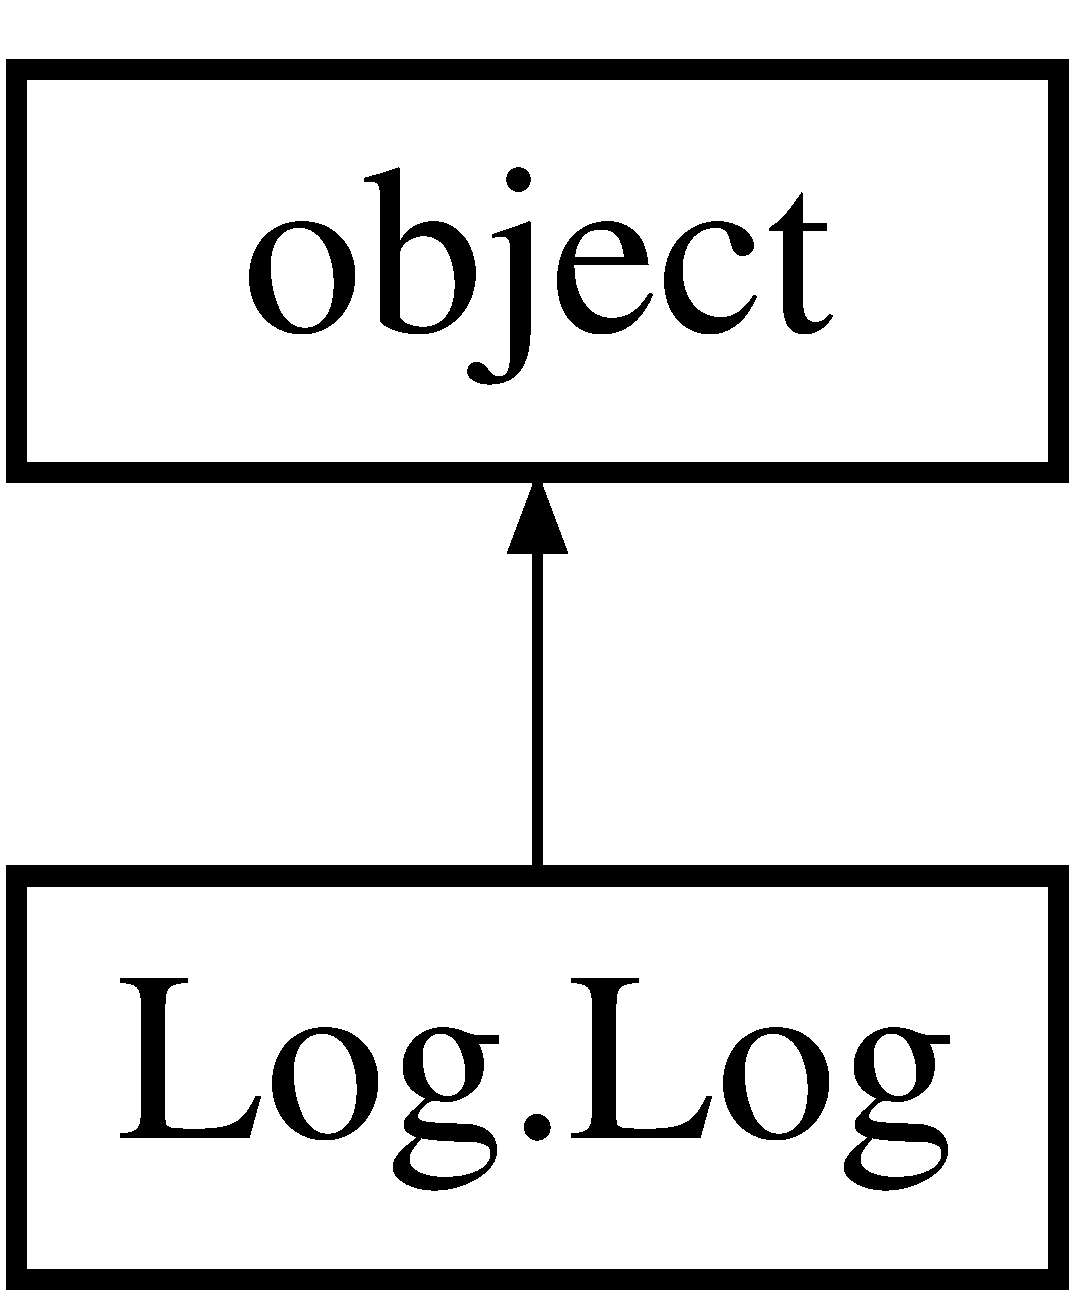
\includegraphics[height=2.000000cm]{class_log_1_1_log}
\end{center}
\end{figure}
\subsection*{Public Member Functions}
\begin{DoxyCompactItemize}
\item 
def \hyperlink{class_log_1_1_log_a67d345cd00f8aa2bccf5a1229b977a94}{\+\_\+\+\_\+init\+\_\+\+\_\+} (self, directory)
\begin{DoxyCompactList}\small\item\em Define 3 differents utils \+: activity.\+log -\/$>$ all activity warning.\+log -\/$>$ only warning error.\+log -\/$>$ error Write all message on terminal too. \end{DoxyCompactList}\item 
def \hyperlink{class_log_1_1_log_ab727696e7af3c67698082458215c2778}{print\+L} (self, p\+Msg, p\+Lvl)
\begin{DoxyCompactList}\small\item\em Add color and write in log with an define level. \end{DoxyCompactList}\end{DoxyCompactItemize}
\subsection*{Public Attributes}
\begin{DoxyCompactItemize}
\item 
\hyperlink{class_log_1_1_log_a0389e51ebd116d483b2b8e662bbcdf09}{logger}
\end{DoxyCompactItemize}


\subsection{Detailed Description}
\hyperlink{class_log_1_1_log}{Log} Manager. 

\subsection{Constructor \& Destructor Documentation}
\hypertarget{class_log_1_1_log_a67d345cd00f8aa2bccf5a1229b977a94}{}\index{Log\+::\+Log@{Log\+::\+Log}!\+\_\+\+\_\+init\+\_\+\+\_\+@{\+\_\+\+\_\+init\+\_\+\+\_\+}}
\index{\+\_\+\+\_\+init\+\_\+\+\_\+@{\+\_\+\+\_\+init\+\_\+\+\_\+}!Log\+::\+Log@{Log\+::\+Log}}
\subsubsection[{\+\_\+\+\_\+init\+\_\+\+\_\+}]{\setlength{\rightskip}{0pt plus 5cm}def Log.\+Log.\+\_\+\+\_\+init\+\_\+\+\_\+ (
\begin{DoxyParamCaption}
\item[{}]{self, }
\item[{}]{directory}
\end{DoxyParamCaption}
)}\label{class_log_1_1_log_a67d345cd00f8aa2bccf5a1229b977a94}


Define 3 differents utils \+: activity.\+log -\/$>$ all activity warning.\+log -\/$>$ only warning error.\+log -\/$>$ error Write all message on terminal too. 



\subsection{Member Function Documentation}
\hypertarget{class_log_1_1_log_ab727696e7af3c67698082458215c2778}{}\index{Log\+::\+Log@{Log\+::\+Log}!print\+L@{print\+L}}
\index{print\+L@{print\+L}!Log\+::\+Log@{Log\+::\+Log}}
\subsubsection[{print\+L}]{\setlength{\rightskip}{0pt plus 5cm}def Log.\+Log.\+print\+L (
\begin{DoxyParamCaption}
\item[{}]{self, }
\item[{}]{p\+Msg, }
\item[{}]{p\+Lvl}
\end{DoxyParamCaption}
)}\label{class_log_1_1_log_ab727696e7af3c67698082458215c2778}


Add color and write in log with an define level. 


\begin{DoxyParams}{Parameters}
{\em p\+Msg} & message to write in log \\
\hline
{\em p\+Lvl} & level of log message \\
\hline
\end{DoxyParams}


\subsection{Member Data Documentation}
\hypertarget{class_log_1_1_log_a0389e51ebd116d483b2b8e662bbcdf09}{}\index{Log\+::\+Log@{Log\+::\+Log}!logger@{logger}}
\index{logger@{logger}!Log\+::\+Log@{Log\+::\+Log}}
\subsubsection[{logger}]{\setlength{\rightskip}{0pt plus 5cm}Log.\+Log.\+logger}\label{class_log_1_1_log_a0389e51ebd116d483b2b8e662bbcdf09}


The documentation for this class was generated from the following file\+:\begin{DoxyCompactItemize}
\item 
/home/sidya/\+Pycharm\+Projects/\+D\+N\+C/serveur/\hyperlink{_log_8py}{Log.\+py}\end{DoxyCompactItemize}

\hypertarget{class_log_1_1lvl}{}\section{Log.\+lvl Class Reference}
\label{class_log_1_1lvl}\index{Log.\+lvl@{Log.\+lvl}}


Define constant value for level utils.  


\subsection*{Static Public Attributes}
\begin{DoxyCompactItemize}
\item 
int \hyperlink{class_log_1_1lvl_a02d1cd2ef3bdac4d2f84facb74452685}{N\+O\+T\+S\+E\+T} = 0
\item 
int \hyperlink{class_log_1_1lvl_abbee3fe06a1896a4bd13d4901f0a892f}{D\+E\+B\+U\+G} = 10
\item 
int \hyperlink{class_log_1_1lvl_af306f6ac0ec77f65ca3a35592b148adb}{I\+N\+F\+O} = 20
\item 
int \hyperlink{class_log_1_1lvl_a453dc11d5d9bdccefd63d5794d9aee47}{W\+A\+R\+N\+I\+N\+G} = 30
\item 
int \hyperlink{class_log_1_1lvl_a9e0eb8280b2ca2279616b80933316159}{F\+A\+I\+L} = 40
\item 
int \hyperlink{class_log_1_1lvl_a3e4b3eb2fc27a260f2971f93758856f2}{C\+R\+I\+T\+I\+C\+A\+L} = 50
\end{DoxyCompactItemize}


\subsection{Detailed Description}
Define constant value for level utils. 

\subsection{Member Data Documentation}
\hypertarget{class_log_1_1lvl_a3e4b3eb2fc27a260f2971f93758856f2}{}\index{Log\+::lvl@{Log\+::lvl}!C\+R\+I\+T\+I\+C\+A\+L@{C\+R\+I\+T\+I\+C\+A\+L}}
\index{C\+R\+I\+T\+I\+C\+A\+L@{C\+R\+I\+T\+I\+C\+A\+L}!Log\+::lvl@{Log\+::lvl}}
\subsubsection[{C\+R\+I\+T\+I\+C\+A\+L}]{\setlength{\rightskip}{0pt plus 5cm}int Log.\+lvl.\+C\+R\+I\+T\+I\+C\+A\+L = 50\hspace{0.3cm}{\ttfamily [static]}}\label{class_log_1_1lvl_a3e4b3eb2fc27a260f2971f93758856f2}
\hypertarget{class_log_1_1lvl_abbee3fe06a1896a4bd13d4901f0a892f}{}\index{Log\+::lvl@{Log\+::lvl}!D\+E\+B\+U\+G@{D\+E\+B\+U\+G}}
\index{D\+E\+B\+U\+G@{D\+E\+B\+U\+G}!Log\+::lvl@{Log\+::lvl}}
\subsubsection[{D\+E\+B\+U\+G}]{\setlength{\rightskip}{0pt plus 5cm}int Log.\+lvl.\+D\+E\+B\+U\+G = 10\hspace{0.3cm}{\ttfamily [static]}}\label{class_log_1_1lvl_abbee3fe06a1896a4bd13d4901f0a892f}
\hypertarget{class_log_1_1lvl_a9e0eb8280b2ca2279616b80933316159}{}\index{Log\+::lvl@{Log\+::lvl}!F\+A\+I\+L@{F\+A\+I\+L}}
\index{F\+A\+I\+L@{F\+A\+I\+L}!Log\+::lvl@{Log\+::lvl}}
\subsubsection[{F\+A\+I\+L}]{\setlength{\rightskip}{0pt plus 5cm}int Log.\+lvl.\+F\+A\+I\+L = 40\hspace{0.3cm}{\ttfamily [static]}}\label{class_log_1_1lvl_a9e0eb8280b2ca2279616b80933316159}
\hypertarget{class_log_1_1lvl_af306f6ac0ec77f65ca3a35592b148adb}{}\index{Log\+::lvl@{Log\+::lvl}!I\+N\+F\+O@{I\+N\+F\+O}}
\index{I\+N\+F\+O@{I\+N\+F\+O}!Log\+::lvl@{Log\+::lvl}}
\subsubsection[{I\+N\+F\+O}]{\setlength{\rightskip}{0pt plus 5cm}int Log.\+lvl.\+I\+N\+F\+O = 20\hspace{0.3cm}{\ttfamily [static]}}\label{class_log_1_1lvl_af306f6ac0ec77f65ca3a35592b148adb}
\hypertarget{class_log_1_1lvl_a02d1cd2ef3bdac4d2f84facb74452685}{}\index{Log\+::lvl@{Log\+::lvl}!N\+O\+T\+S\+E\+T@{N\+O\+T\+S\+E\+T}}
\index{N\+O\+T\+S\+E\+T@{N\+O\+T\+S\+E\+T}!Log\+::lvl@{Log\+::lvl}}
\subsubsection[{N\+O\+T\+S\+E\+T}]{\setlength{\rightskip}{0pt plus 5cm}int Log.\+lvl.\+N\+O\+T\+S\+E\+T = 0\hspace{0.3cm}{\ttfamily [static]}}\label{class_log_1_1lvl_a02d1cd2ef3bdac4d2f84facb74452685}
\hypertarget{class_log_1_1lvl_a453dc11d5d9bdccefd63d5794d9aee47}{}\index{Log\+::lvl@{Log\+::lvl}!W\+A\+R\+N\+I\+N\+G@{W\+A\+R\+N\+I\+N\+G}}
\index{W\+A\+R\+N\+I\+N\+G@{W\+A\+R\+N\+I\+N\+G}!Log\+::lvl@{Log\+::lvl}}
\subsubsection[{W\+A\+R\+N\+I\+N\+G}]{\setlength{\rightskip}{0pt plus 5cm}int Log.\+lvl.\+W\+A\+R\+N\+I\+N\+G = 30\hspace{0.3cm}{\ttfamily [static]}}\label{class_log_1_1lvl_a453dc11d5d9bdccefd63d5794d9aee47}


The documentation for this class was generated from the following file\+:\begin{DoxyCompactItemize}
\item 
/home/sidya/\+Pycharm\+Projects/\+D\+N\+C/serveur/\hyperlink{_log_8py}{Log.\+py}\end{DoxyCompactItemize}

\hypertarget{class_log_1_1_single_level_filter}{}\section{Log.\+Single\+Level\+Filter Class Reference}
\label{class_log_1_1_single_level_filter}\index{Log.\+Single\+Level\+Filter@{Log.\+Single\+Level\+Filter}}


Filter for one level.  


Inheritance diagram for Log.\+Single\+Level\+Filter\+:\begin{figure}[H]
\begin{center}
\leavevmode
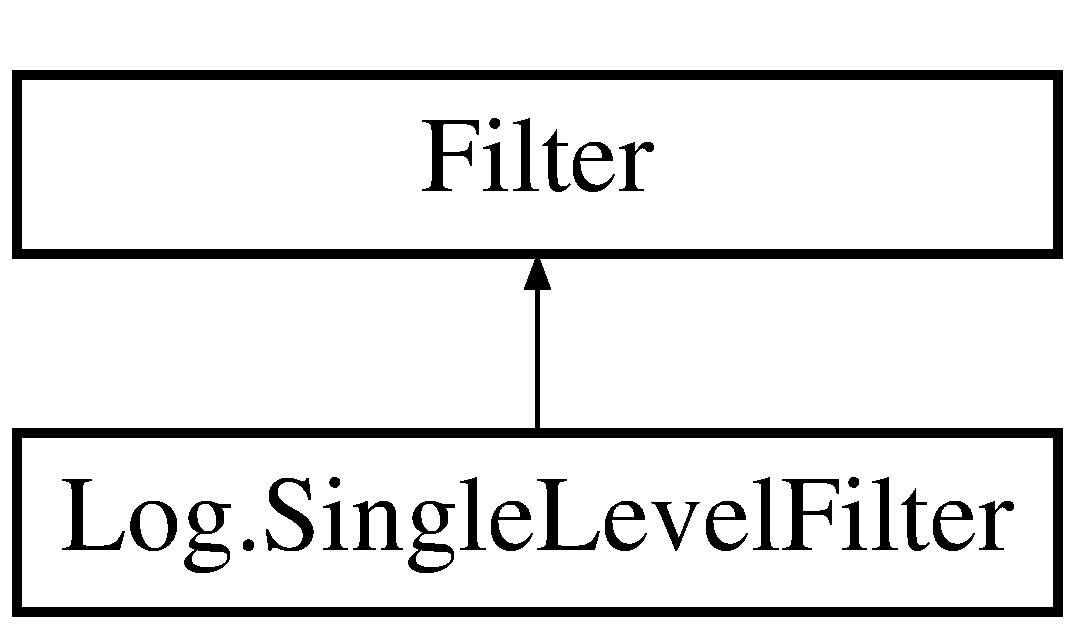
\includegraphics[height=2.000000cm]{class_log_1_1_single_level_filter}
\end{center}
\end{figure}
\subsection*{Public Member Functions}
\begin{DoxyCompactItemize}
\item 
def \hyperlink{class_log_1_1_single_level_filter_aeaf022ddb4e62a8147a1867399d5b6c7}{\+\_\+\+\_\+init\+\_\+\+\_\+} (self, \hyperlink{class_log_1_1_single_level_filter_abae072b8db802c0e4c4ab15823020916}{passlevel}, \hyperlink{class_log_1_1_single_level_filter_a4a0c91f813f78d0f28435283661c44c7}{reject})
\begin{DoxyCompactList}\small\item\em Constructor. \end{DoxyCompactList}\item 
def \hyperlink{class_log_1_1_single_level_filter_a0bf970b79dca04f61fe488eb0f8314ee}{filter} (self, record)
\end{DoxyCompactItemize}
\subsection*{Public Attributes}
\begin{DoxyCompactItemize}
\item 
\hyperlink{class_log_1_1_single_level_filter_abae072b8db802c0e4c4ab15823020916}{passlevel}
\item 
\hyperlink{class_log_1_1_single_level_filter_a4a0c91f813f78d0f28435283661c44c7}{reject}
\end{DoxyCompactItemize}


\subsection{Detailed Description}
Filter for one level. 

\begin{DoxyVerb}\end{DoxyVerb}
 

\subsection{Constructor \& Destructor Documentation}
\hypertarget{class_log_1_1_single_level_filter_aeaf022ddb4e62a8147a1867399d5b6c7}{}\index{Log\+::\+Single\+Level\+Filter@{Log\+::\+Single\+Level\+Filter}!\+\_\+\+\_\+init\+\_\+\+\_\+@{\+\_\+\+\_\+init\+\_\+\+\_\+}}
\index{\+\_\+\+\_\+init\+\_\+\+\_\+@{\+\_\+\+\_\+init\+\_\+\+\_\+}!Log\+::\+Single\+Level\+Filter@{Log\+::\+Single\+Level\+Filter}}
\subsubsection[{\+\_\+\+\_\+init\+\_\+\+\_\+}]{\setlength{\rightskip}{0pt plus 5cm}def Log.\+Single\+Level\+Filter.\+\_\+\+\_\+init\+\_\+\+\_\+ (
\begin{DoxyParamCaption}
\item[{}]{self, }
\item[{}]{passlevel, }
\item[{}]{reject}
\end{DoxyParamCaption}
)}\label{class_log_1_1_single_level_filter_aeaf022ddb4e62a8147a1867399d5b6c7}


Constructor. 


\begin{DoxyParams}{Parameters}
{\em passlevel} & level to filter \\
\hline
{\em reject} & true on reject state \\
\hline
\end{DoxyParams}


\subsection{Member Function Documentation}
\hypertarget{class_log_1_1_single_level_filter_a0bf970b79dca04f61fe488eb0f8314ee}{}\index{Log\+::\+Single\+Level\+Filter@{Log\+::\+Single\+Level\+Filter}!filter@{filter}}
\index{filter@{filter}!Log\+::\+Single\+Level\+Filter@{Log\+::\+Single\+Level\+Filter}}
\subsubsection[{filter}]{\setlength{\rightskip}{0pt plus 5cm}def Log.\+Single\+Level\+Filter.\+filter (
\begin{DoxyParamCaption}
\item[{}]{self, }
\item[{}]{record}
\end{DoxyParamCaption}
)}\label{class_log_1_1_single_level_filter_a0bf970b79dca04f61fe488eb0f8314ee}


\subsection{Member Data Documentation}
\hypertarget{class_log_1_1_single_level_filter_abae072b8db802c0e4c4ab15823020916}{}\index{Log\+::\+Single\+Level\+Filter@{Log\+::\+Single\+Level\+Filter}!passlevel@{passlevel}}
\index{passlevel@{passlevel}!Log\+::\+Single\+Level\+Filter@{Log\+::\+Single\+Level\+Filter}}
\subsubsection[{passlevel}]{\setlength{\rightskip}{0pt plus 5cm}Log.\+Single\+Level\+Filter.\+passlevel}\label{class_log_1_1_single_level_filter_abae072b8db802c0e4c4ab15823020916}
\hypertarget{class_log_1_1_single_level_filter_a4a0c91f813f78d0f28435283661c44c7}{}\index{Log\+::\+Single\+Level\+Filter@{Log\+::\+Single\+Level\+Filter}!reject@{reject}}
\index{reject@{reject}!Log\+::\+Single\+Level\+Filter@{Log\+::\+Single\+Level\+Filter}}
\subsubsection[{reject}]{\setlength{\rightskip}{0pt plus 5cm}Log.\+Single\+Level\+Filter.\+reject}\label{class_log_1_1_single_level_filter_a4a0c91f813f78d0f28435283661c44c7}


The documentation for this class was generated from the following file\+:\begin{DoxyCompactItemize}
\item 
/home/sidya/\+Pycharm\+Projects/\+D\+N\+C/serveur/\hyperlink{_log_8py}{Log.\+py}\end{DoxyCompactItemize}

\chapter{File Documentation}
\hypertarget{_log_8py}{}\section{/home/sidya/\+Pycharm\+Projects/\+D\+N\+C/serveur/\+Log.py File Reference}
\label{_log_8py}\index{/home/sidya/\+Pycharm\+Projects/\+D\+N\+C/serveur/\+Log.\+py@{/home/sidya/\+Pycharm\+Projects/\+D\+N\+C/serveur/\+Log.\+py}}
\subsection*{Classes}
\begin{DoxyCompactItemize}
\item 
class \hyperlink{class_log_1_1bcolors}{Log.\+bcolors}
\begin{DoxyCompactList}\small\item\em Define constant color value for different level. \end{DoxyCompactList}\item 
class \hyperlink{class_log_1_1lvl}{Log.\+lvl}
\begin{DoxyCompactList}\small\item\em Define constant value for level utils. \end{DoxyCompactList}\item 
class \hyperlink{class_log_1_1_single_level_filter}{Log.\+Single\+Level\+Filter}
\begin{DoxyCompactList}\small\item\em Filter for one level. \end{DoxyCompactList}\item 
class \hyperlink{class_log_1_1_log}{Log.\+Log}
\begin{DoxyCompactList}\small\item\em \hyperlink{class_log_1_1_log}{Log} Manager. \end{DoxyCompactList}\end{DoxyCompactItemize}
\subsection*{Namespaces}
\begin{DoxyCompactItemize}
\item 
 \hyperlink{namespace_log}{Log}
\begin{DoxyCompactList}\small\item\em Module \hyperlink{namespace_log}{Log}. \end{DoxyCompactList}\end{DoxyCompactItemize}

\hypertarget{_r_e_a_d_m_e_8md}{}\section{/home/sidya/\+Pycharm\+Projects/\+D\+N\+C/serveur/\+R\+E\+A\+D\+M\+E.md File Reference}
\label{_r_e_a_d_m_e_8md}\index{/home/sidya/\+Pycharm\+Projects/\+D\+N\+C/serveur/\+R\+E\+A\+D\+M\+E.\+md@{/home/sidya/\+Pycharm\+Projects/\+D\+N\+C/serveur/\+R\+E\+A\+D\+M\+E.\+md}}

\hypertarget{_server_8py}{}\section{/home/sidya/\+Pycharm\+Projects/\+D\+N\+C/serveur/\+Server.py File Reference}
\label{_server_8py}\index{/home/sidya/\+Pycharm\+Projects/\+D\+N\+C/serveur/\+Server.\+py@{/home/sidya/\+Pycharm\+Projects/\+D\+N\+C/serveur/\+Server.\+py}}
\subsection*{Namespaces}
\begin{DoxyCompactItemize}
\item 
 \hyperlink{namespace_server}{Server}
\begin{DoxyCompactList}\small\item\em Module server. \end{DoxyCompactList}\end{DoxyCompactItemize}
\subsection*{Functions}
\begin{DoxyCompactItemize}
\item 
def \hyperlink{namespace_server_a3b6f7f7679d98f214467d05da4618a0c}{Server.\+main} ()
\begin{DoxyCompactList}\small\item\em Load Configuration and Start the \hyperlink{namespace_server}{Server}. \end{DoxyCompactList}\item 
def \hyperlink{namespace_server_a5956f54107dc04f2c1700fcf62f1afc9}{Server.\+handle\+\_\+connection} (connection, client\+\_\+address)
\begin{DoxyCompactList}\small\item\em Handle a connection from a client. \end{DoxyCompactList}\item 
def \hyperlink{namespace_server_a8965f4e84689d4e2b198091f0383fd41}{Server.\+handle\+\_\+request} (connection, data)
\begin{DoxyCompactList}\small\item\em Handle a request. \end{DoxyCompactList}\item 
def \hyperlink{namespace_server_a5b7286b84051e8f089e78cec5276027f}{Server.\+broadcast\+\_\+message} (connection, message)
\begin{DoxyCompactList}\small\item\em Broadcast a message to all the users connected except to the sender of the request. \end{DoxyCompactList}\item 
def \hyperlink{namespace_server_a79e61c36bfba574632384d7c95f687e8}{Server.\+user\+\_\+list\+\_\+active} (connection)
\begin{DoxyCompactList}\small\item\em Send the list of enable user. \end{DoxyCompactList}\item 
def \hyperlink{namespace_server_a616374a08f1e1cd1c4fa745e10af349a}{Server.\+user\+\_\+list\+\_\+away} (connection)
\begin{DoxyCompactList}\small\item\em Send the list of disable user. \end{DoxyCompactList}\item 
def \hyperlink{namespace_server_a59bc6f10d51dddca1906c85fdac1cc62}{Server.\+change\+\_\+name} (connection, pseudo)
\begin{DoxyCompactList}\small\item\em Change the nickname of the user. \end{DoxyCompactList}\item 
def \hyperlink{namespace_server_aedccc2662d6bc5892f70e48009ed1b59}{Server.\+new\+\_\+name} (connection, pseudo)
\begin{DoxyCompactList}\small\item\em Affect the nickname of the user for the first time. \end{DoxyCompactList}\item 
def \hyperlink{namespace_server_a46ba24f249f2961ada72160f9a9ba9b8}{Server.\+ask\+\_\+private\+\_\+message} (connection, pseudo)
\begin{DoxyCompactList}\small\item\em Ask for a private discussion between the sender of the request and the pseudo. \end{DoxyCompactList}\item 
def \hyperlink{namespace_server_a1879fdb42898934db420d6c225db536e}{Server.\+accept\+\_\+private\+\_\+message} (connection, pseudo)
\begin{DoxyCompactList}\small\item\em Accept a private discussion. \end{DoxyCompactList}\item 
def \hyperlink{namespace_server_a1ccbd55ee3033925a2b1ef2716dd0829}{Server.\+reject\+\_\+private\+\_\+message} (connection, pseudo)
\begin{DoxyCompactList}\small\item\em Reject a private discussion. \end{DoxyCompactList}\item 
def \hyperlink{namespace_server_a5605c682f147e7cf9018ac02bb089989}{Server.\+private\+\_\+message} (connection, pseudo, msg)
\begin{DoxyCompactList}\small\item\em Send a private message if a private discussion had been accepted. \end{DoxyCompactList}\item 
def \hyperlink{namespace_server_a2ddcf35a85844615fa31e72f6dcc52b0}{Server.\+ask\+\_\+file} (connection, pseudo, file)
\begin{DoxyCompactList}\small\item\em Ask for a file transfer between the sender of the request and the pseudo. \end{DoxyCompactList}\item 
def \hyperlink{namespace_server_a0f21810c2b82ea1a98725185d2f3a70a}{Server.\+accept\+\_\+file} (connection, pseudo, file, port)
\begin{DoxyCompactList}\small\item\em Accept a file transfer. \end{DoxyCompactList}\item 
def \hyperlink{namespace_server_a7b5be6de60d79f607c206c3675166301}{Server.\+reject\+\_\+file} (connection, pseudo, file)
\begin{DoxyCompactList}\small\item\em Reject a file transfer. \end{DoxyCompactList}\item 
def \hyperlink{namespace_server_a114698f1955c3ff109f9fbbc1df306fa}{Server.\+enable\+\_\+user} (connection)
\begin{DoxyCompactList}\small\item\em Enable user. \end{DoxyCompactList}\item 
def \hyperlink{namespace_server_af20de30ab901173d2bc8f58da7c05c25}{Server.\+disable\+\_\+user} (connection)
\begin{DoxyCompactList}\small\item\em Disable user. \end{DoxyCompactList}\item 
def \hyperlink{namespace_server_af73d203b1f93b0f4014456fb52c7626a}{Server.\+quit\+\_\+user} (connection)
\begin{DoxyCompactList}\small\item\em Disconnect user. \end{DoxyCompactList}\item 
def \hyperlink{namespace_server_a23b4ef94218cf46a4a1af4ed37c5278b}{Server.\+get\+\_\+connection\+\_\+by\+\_\+pseudo} (pseudo)
\begin{DoxyCompactList}\small\item\em Get the socket descriptor by a pseudo. \end{DoxyCompactList}\end{DoxyCompactItemize}
\subsection*{Variables}
\begin{DoxyCompactItemize}
\item 
int \hyperlink{namespace_server_ad80a48b2e2123c1442355c35e9a12180}{Server.\+U\+S\+E\+R\+L\+I\+S\+T\+\_\+\+E\+N\+A\+B\+L\+E} = 300
\item 
int \hyperlink{namespace_server_a20a80092be74432cb9d70ee7d69a7897}{Server.\+U\+S\+E\+R\+L\+I\+S\+T\+\_\+\+D\+I\+S\+A\+B\+L\+E} = 301
\item 
int \hyperlink{namespace_server_a6d93191ccb1aca72fc4e4c35df44dc54}{Server.\+H\+A\+S\+\_\+\+J\+O\+I\+N} = 302
\item 
int \hyperlink{namespace_server_a30d806240b31876a27ec926941c45c7b}{Server.\+H\+A\+S\+\_\+\+L\+E\+F\+T} = 303
\item 
int \hyperlink{namespace_server_a6403a5757be6c8ca9123c4a1d84fcf8f}{Server.\+N\+E\+W\+\_\+\+M\+S\+G} = 304
\item 
int \hyperlink{namespace_server_a74a7d4ecad24b92d3e58fa6935bf4738}{Server.\+N\+A\+M\+E\+\_\+\+C\+H\+A\+N\+G\+E\+D} = 305
\item 
int \hyperlink{namespace_server_a5baa396c48e11763e3a9e6b7949c848c}{Server.\+N\+E\+W\+\_\+\+P\+M} = 306
\item 
int \hyperlink{namespace_server_a0a4c647255674a0b8b88b4e0352735b8}{Server.\+A\+S\+K\+I\+N\+G\+\_\+\+F\+O\+R\+\_\+\+P\+M} = 307
\item 
int \hyperlink{namespace_server_a7ed9c5c7a5d63ed69e59b8e1facf1941}{Server.\+P\+R\+I\+V\+A\+T\+E\+\_\+\+D\+I\+S\+C\+U\+\_\+\+A\+C\+C\+E\+P\+T\+E\+D\+\_\+\+F\+R\+O\+M} = 308
\item 
int \hyperlink{namespace_server_a1893bf20254e625ee4d337b5ac4c0c7c}{Server.\+P\+R\+I\+V\+A\+T\+E\+\_\+\+D\+I\+S\+C\+U\+\_\+\+R\+E\+F\+U\+S\+E\+D\+\_\+\+F\+R\+O\+M} = 309
\item 
int \hyperlink{namespace_server_a706046d1323e6c8efcf412f039468feb}{Server.\+I\+S\+\_\+\+N\+O\+W\+\_\+\+E\+N\+A\+B\+L\+E} = 310
\item 
int \hyperlink{namespace_server_ad86289daa647c23b114d6eeecb311b74}{Server.\+I\+S\+\_\+\+N\+O\+W\+\_\+\+D\+I\+S\+A\+B\+L\+E} = 311
\item 
int \hyperlink{namespace_server_a948cf317958301749b5133cb0e429cbf}{Server.\+H\+A\+S\+\_\+\+A\+S\+K\+E\+D\+\_\+\+F\+I\+L\+E} = 312
\item 
int \hyperlink{namespace_server_a0e574da7da6c6fa749d02202b36efae4}{Server.\+C\+A\+N\+\_\+\+S\+E\+N\+D\+\_\+\+F\+I\+L\+E} = 313
\item 
int \hyperlink{namespace_server_ac45d5a8294d066cceee3b4f808f4ab04}{Server.\+H\+A\+S\+\_\+\+R\+E\+J\+E\+C\+T\+\_\+\+F\+I\+L\+E} = 314
\item 
int \hyperlink{namespace_server_a0a446eb75138a1b946c7adf06feaa638}{Server.\+S\+U\+C\+C\+\_\+\+C\+H\+A\+N\+N\+E\+L\+\_\+\+J\+O\+I\+N\+E\+D} = 200
\item 
int \hyperlink{namespace_server_a9653741644804867d5c762d637aa714a}{Server.\+S\+U\+C\+C\+\_\+\+C\+H\+A\+N\+N\+E\+L\+\_\+\+Q\+U\+I\+T} = 201
\item 
int \hyperlink{namespace_server_ae41a5af03180af57ac7842e0309d4fa7}{Server.\+S\+U\+C\+C\+\_\+\+M\+E\+S\+S\+A\+G\+E\+\_\+\+S\+E\+N\+D\+E\+D} = 202
\item 
int \hyperlink{namespace_server_a48248ec155d0641a5e47603f2b63b37f}{Server.\+S\+U\+C\+C\+\_\+\+N\+I\+C\+K\+N\+A\+M\+E\+\_\+\+C\+H\+A\+N\+G\+E\+D} = 203
\item 
int \hyperlink{namespace_server_a01ffc4404f384ae4ca5ef739be4abacd}{Server.\+S\+U\+C\+C\+\_\+\+P\+M\+\_\+\+S\+E\+N\+D\+E\+D} = 205
\item 
int \hyperlink{namespace_server_a44b9c60be4a9b7cb3840d7cf13a2ef07}{Server.\+S\+U\+C\+C\+E\+S\+S\+F\+U\+L\+\_\+\+A\+S\+K\+E\+D\+\_\+\+C\+O\+N\+V} = 206
\item 
int \hyperlink{namespace_server_a9f976ad2360614ad56f0f9b69e1d5531}{Server.\+S\+U\+C\+C\+E\+S\+S\+F\+U\+L\+\_\+\+A\+C\+C\+E\+P\+T\+E\+D\+\_\+\+C\+O\+N\+V} = 207
\item 
int \hyperlink{namespace_server_a70f0f7aa86090898f53d0f52d3f4e4d7}{Server.\+S\+U\+C\+C\+E\+S\+S\+F\+U\+L\+\_\+\+R\+E\+F\+U\+S\+E\+D\+\_\+\+C\+O\+N\+V} = 208
\item 
int \hyperlink{namespace_server_a0d04d348838bfae170d279430a2570df}{Server.\+S\+U\+C\+C\+\_\+\+E\+N\+A\+B\+L\+E\+D} = 209
\item 
int \hyperlink{namespace_server_a662b6a6d59fdbe98f37a4dac857f56e6}{Server.\+S\+U\+C\+C\+\_\+\+D\+I\+S\+A\+B\+L\+E\+D} = 210
\item 
int \hyperlink{namespace_server_a0f9d2f56d8da4e1f082db5b399c53e49}{Server.\+S\+U\+C\+C\+\_\+\+P\+M\+F\+I\+L\+E} = 211
\item 
int \hyperlink{namespace_server_a53415d85b058622e3aae5ce84985d5ce}{Server.\+S\+U\+C\+C\+\_\+\+A\+C\+C\+E\+P\+T\+E\+D\+\_\+\+F\+I\+L\+E} = 212
\item 
int \hyperlink{namespace_server_aaaad6f296a49912bba515f1035d9af89}{Server.\+S\+U\+C\+C\+\_\+\+R\+E\+F\+U\+S\+E\+D\+\_\+\+F\+I\+L\+E} = 213
\item 
int \hyperlink{namespace_server_a694f8f0d80fb62bdbe88484506f798e9}{Server.\+E\+R\+R\+\_\+\+N\+I\+C\+K\+N\+A\+M\+E\+\_\+\+A\+L\+R\+E\+A\+D\+Y\+\_\+\+U\+S\+E\+D} = 400
\item 
int \hyperlink{namespace_server_ac38a41cef46c16cd55f914479173d7e7}{Server.\+E\+R\+R\+\_\+\+N\+O\+\_\+\+N\+I\+C\+K\+N\+A\+M\+E} = 401
\item 
int \hyperlink{namespace_server_a4a2b6adb4d445ae828f03ab00e99024b}{Server.\+E\+R\+R\+\_\+\+C\+O\+N\+V\+\_\+\+N\+O\+T\+\_\+\+A\+L\+L\+O\+W\+E\+D} = 402
\item 
int \hyperlink{namespace_server_a58ccc0de13c1317e02ae6c7acc95babd}{Server.\+D\+E\+S\+T\+\_\+\+N\+O\+T\+\_\+\+F\+O\+U\+N\+D} = 403
\item 
int \hyperlink{namespace_server_a3636d43b6ad3b3f41bf531830f567577}{Server.\+E\+R\+R\+\_\+\+A\+L\+R\+E\+A\+D\+Y\+\_\+\+A\+S\+K\+E\+D\+\_\+\+F\+O\+R\+\_\+\+P\+M} = 404
\item 
int \hyperlink{namespace_server_a64e45a54c72b15ec3ef27064a69067bf}{Server.\+E\+R\+R\+\_\+\+N\+O\+\_\+\+I\+N\+V\+I\+T\+\_\+\+T\+O\+\_\+\+C\+O\+N\+V\+\_\+\+F\+O\+U\+N\+D} = 405
\item 
int \hyperlink{namespace_server_ad7305f8755fe9025d1a08d7e28931fff}{Server.\+E\+R\+R\+\_\+\+U\+N\+K\+N\+O\+W\+N\+\_\+\+A\+C\+C\+E\+P\+T\+E\+D\+\_\+\+F\+I\+L\+E} = 406
\item 
int \hyperlink{namespace_server_accfadc084947316e3de1bf2e8f0292de}{Server.\+C\+O\+M\+M\+A\+N\+D\+\_\+\+N\+O\+T\+\_\+\+F\+O\+U\+N\+D} = 407
\item 
int \hyperlink{namespace_server_a8a68f5e3a20d872bc0a0657c42e2281d}{Server.\+E\+R\+R\+\_\+\+I\+N\+V\+A\+L\+I\+D\+\_\+\+N\+I\+C\+K\+N\+A\+M\+E} = 408
\item 
int \hyperlink{namespace_server_a3515074e422119d92e2f6a0087eda6a9}{Server.\+E\+R\+R\+\_\+\+I\+N\+T\+E\+R\+N\+A\+L\+\_\+\+S\+E\+R\+V\+E\+R\+\_\+\+E\+R\+R\+O\+R} = 409
\item 
int \hyperlink{namespace_server_a03d76767907390977f2f88588ddb2e46}{Server.\+E\+R\+R\+\_\+\+N\+O\+T\+\_\+\+D\+I\+S\+A\+B\+L\+E\+D} = 410
\item 
int \hyperlink{namespace_server_acc557207eefe9a375185ff17a8f4c641}{Server.\+E\+R\+R\+\_\+\+N\+O\+T\+\_\+\+E\+N\+A\+B\+L\+E\+D} = 411
\end{DoxyCompactItemize}

%--- End generated contents ---

% Index
\backmatter
\newpage
\phantomsection
\clearemptydoublepage
\addcontentsline{toc}{chapter}{Index}
\printindex

\end{document}
